\section{Design}

\subsection{Styleguide}

\subsubsection*{Skrifttyper}

Appen bruger skrifttypen Roboto Condensed \footcite{roboto-condensed} til al tekst.

\begin{figure}[H]
    \label{font}
    \centering
    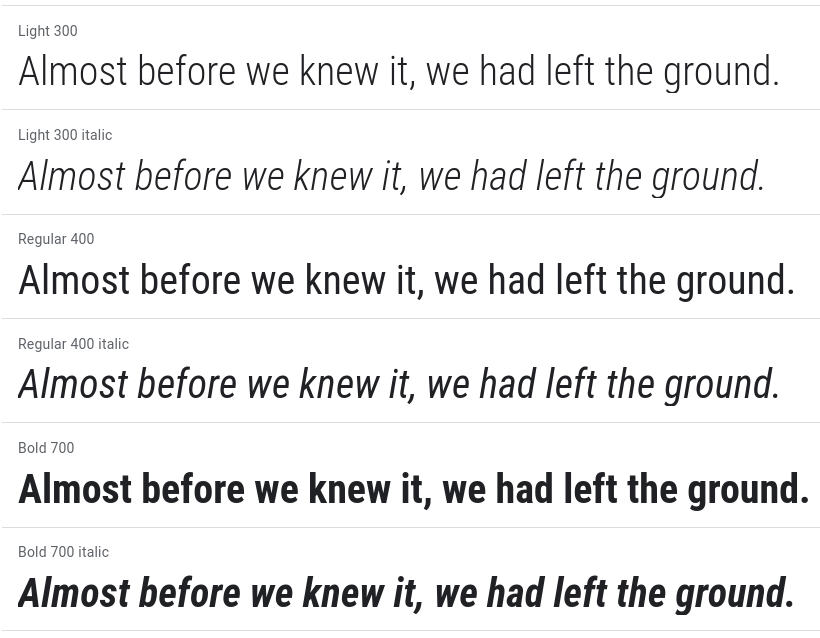
\includegraphics[width=1\textwidth]{img/s1-11.png}
    \caption{Roboto font}
\end{figure}

\subsubsection*{Farver}

Farverne tager udgangspunkt i farver som man tit møder, når man arbejder med planter. F.eks. repræsenterer grøn planter og jordfarverne potter og jord.

Begge farveskemaer er udvalgt af en professionel xxxx, og vi har valgt at bruge det øverste, for at have lidt varmere toner i appen.

\begin{figure}[H]
    \label{farver}
    \centering
    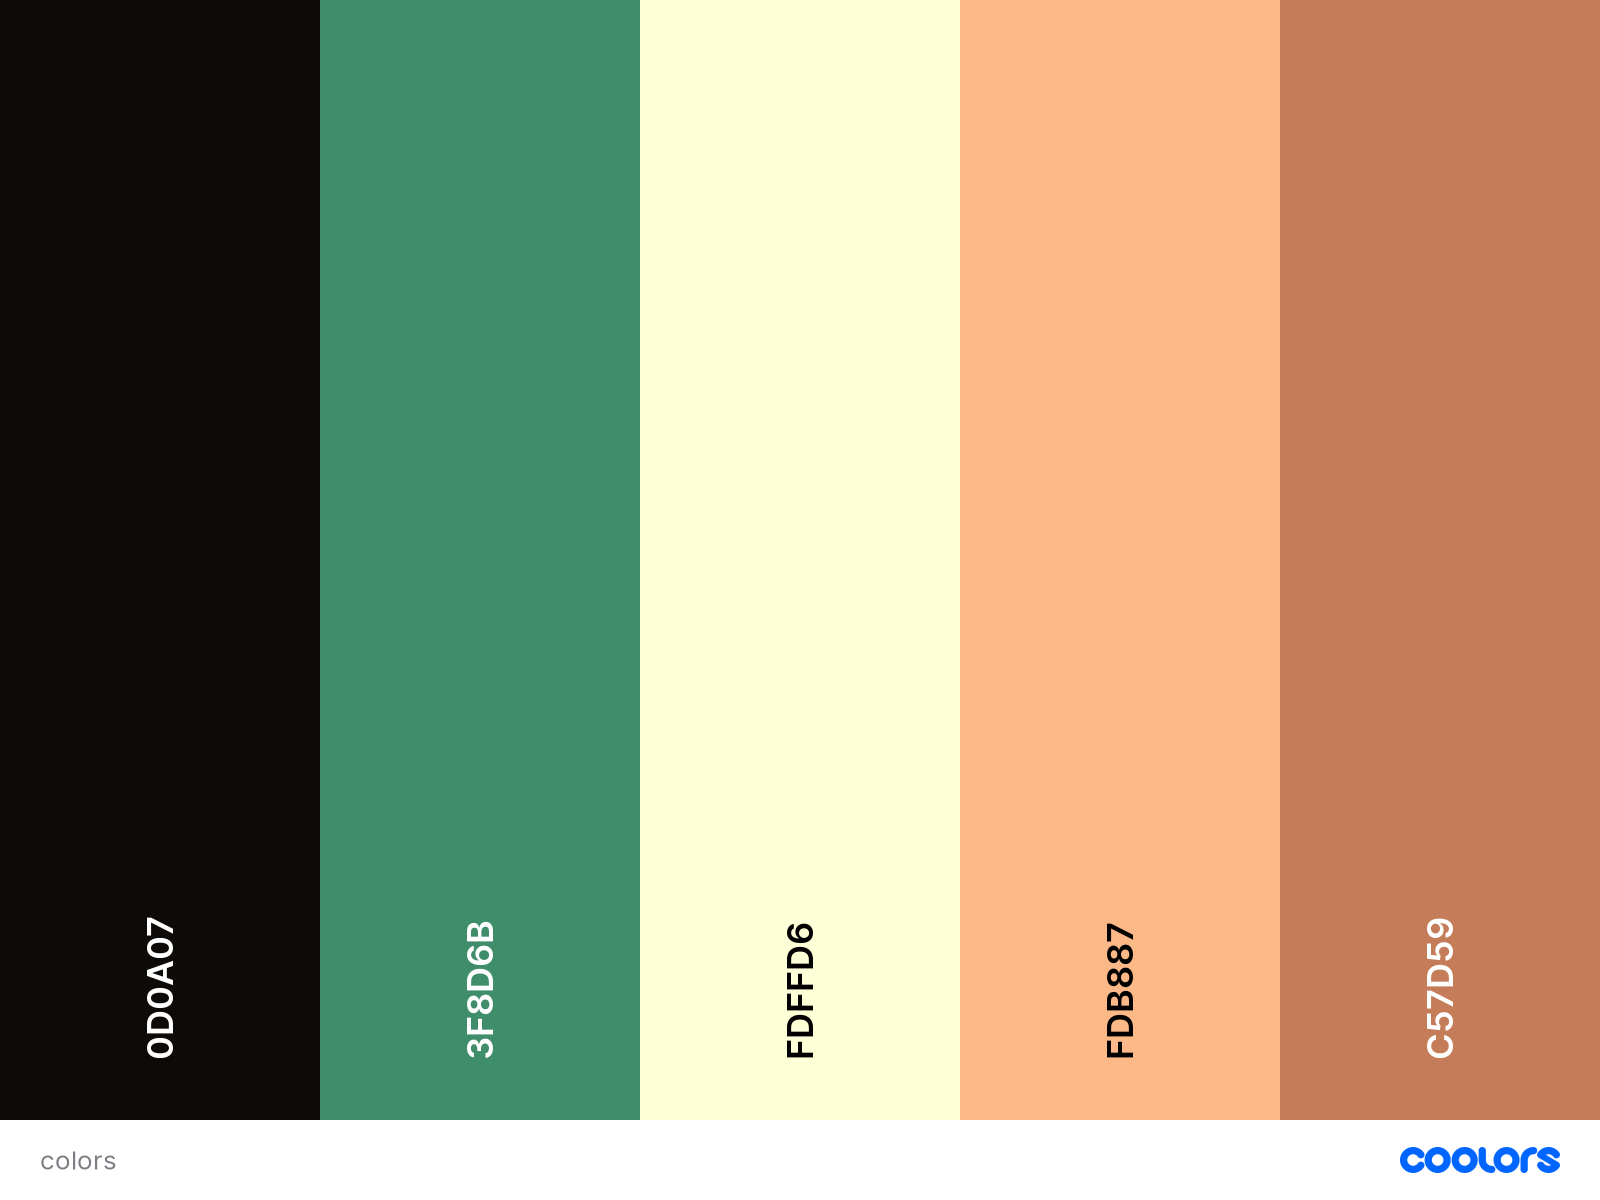
\includegraphics[width=0.7\textwidth]{img/colors.png}
    \caption{Appfarver}
\end{figure}

\subsubsection*{Textstørrelser}

\begin{itemize}
    \item 10
    \item 16
    \item 24
    \item 36
\end{itemize}

\subsubsection*{Padding og margener}

\begin{itemize}
    \item 5
    \item 10
    \item 15
    \item 20
\end{itemize}

\subsection{Sketches}

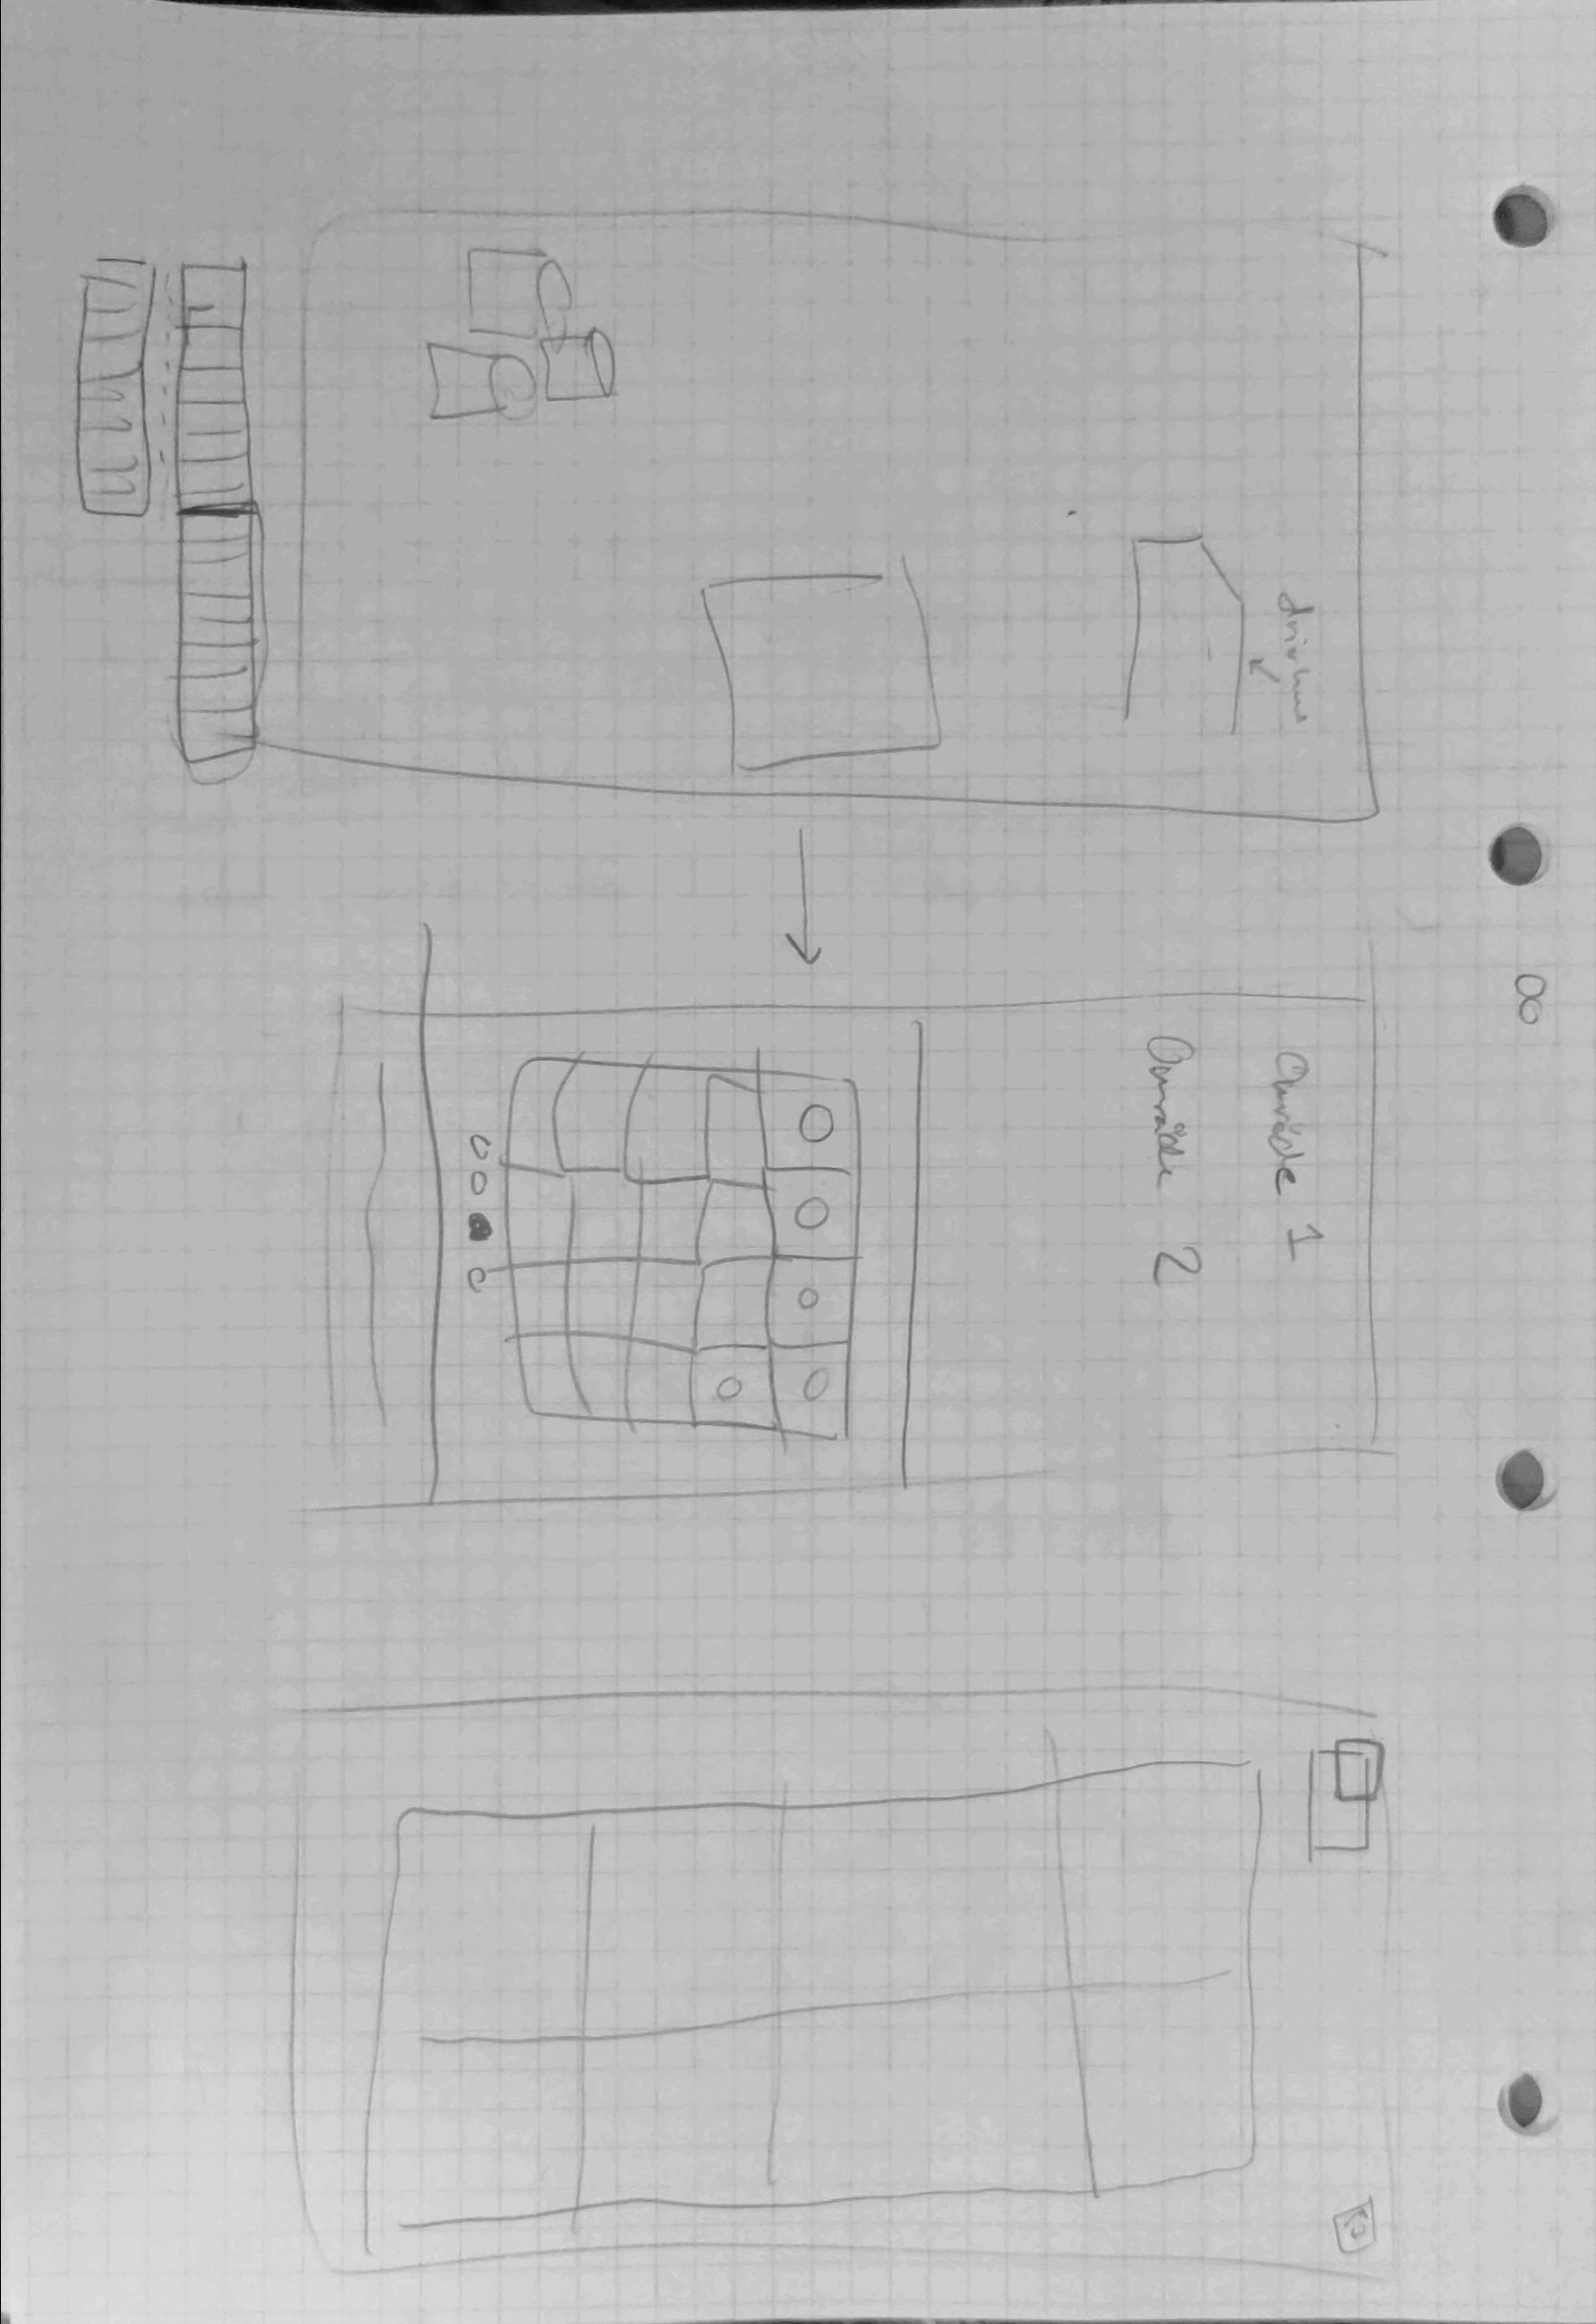
\includegraphics[width=1\textwidth]{img/s1-1.jpg}\\
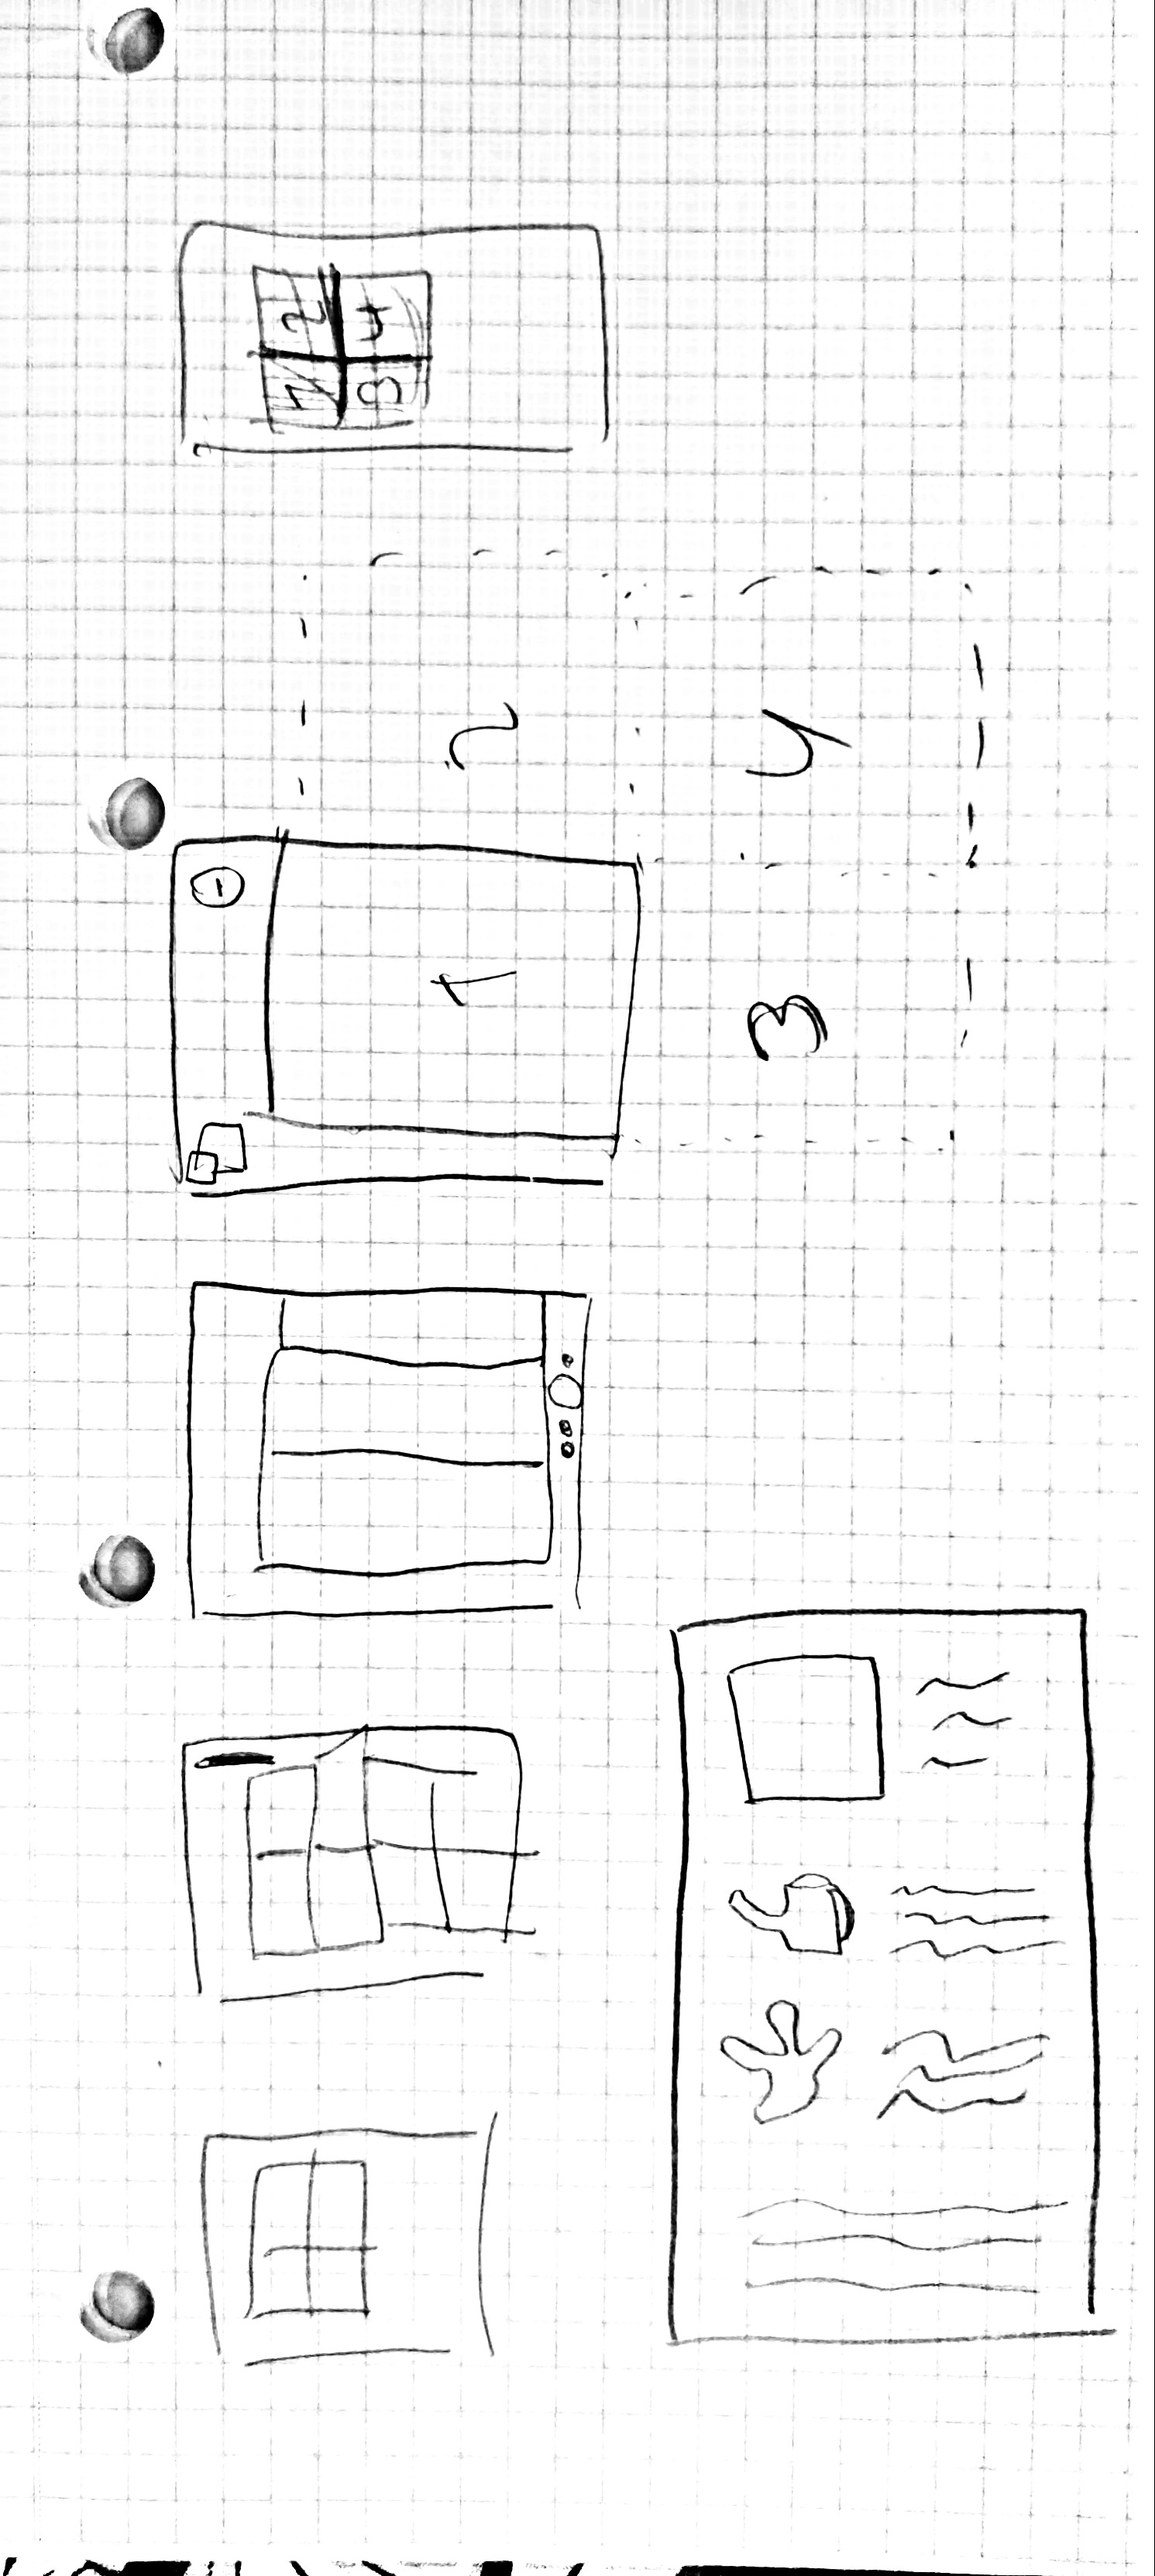
\includegraphics[width=1\textwidth]{img/s1-3.jpg}\\
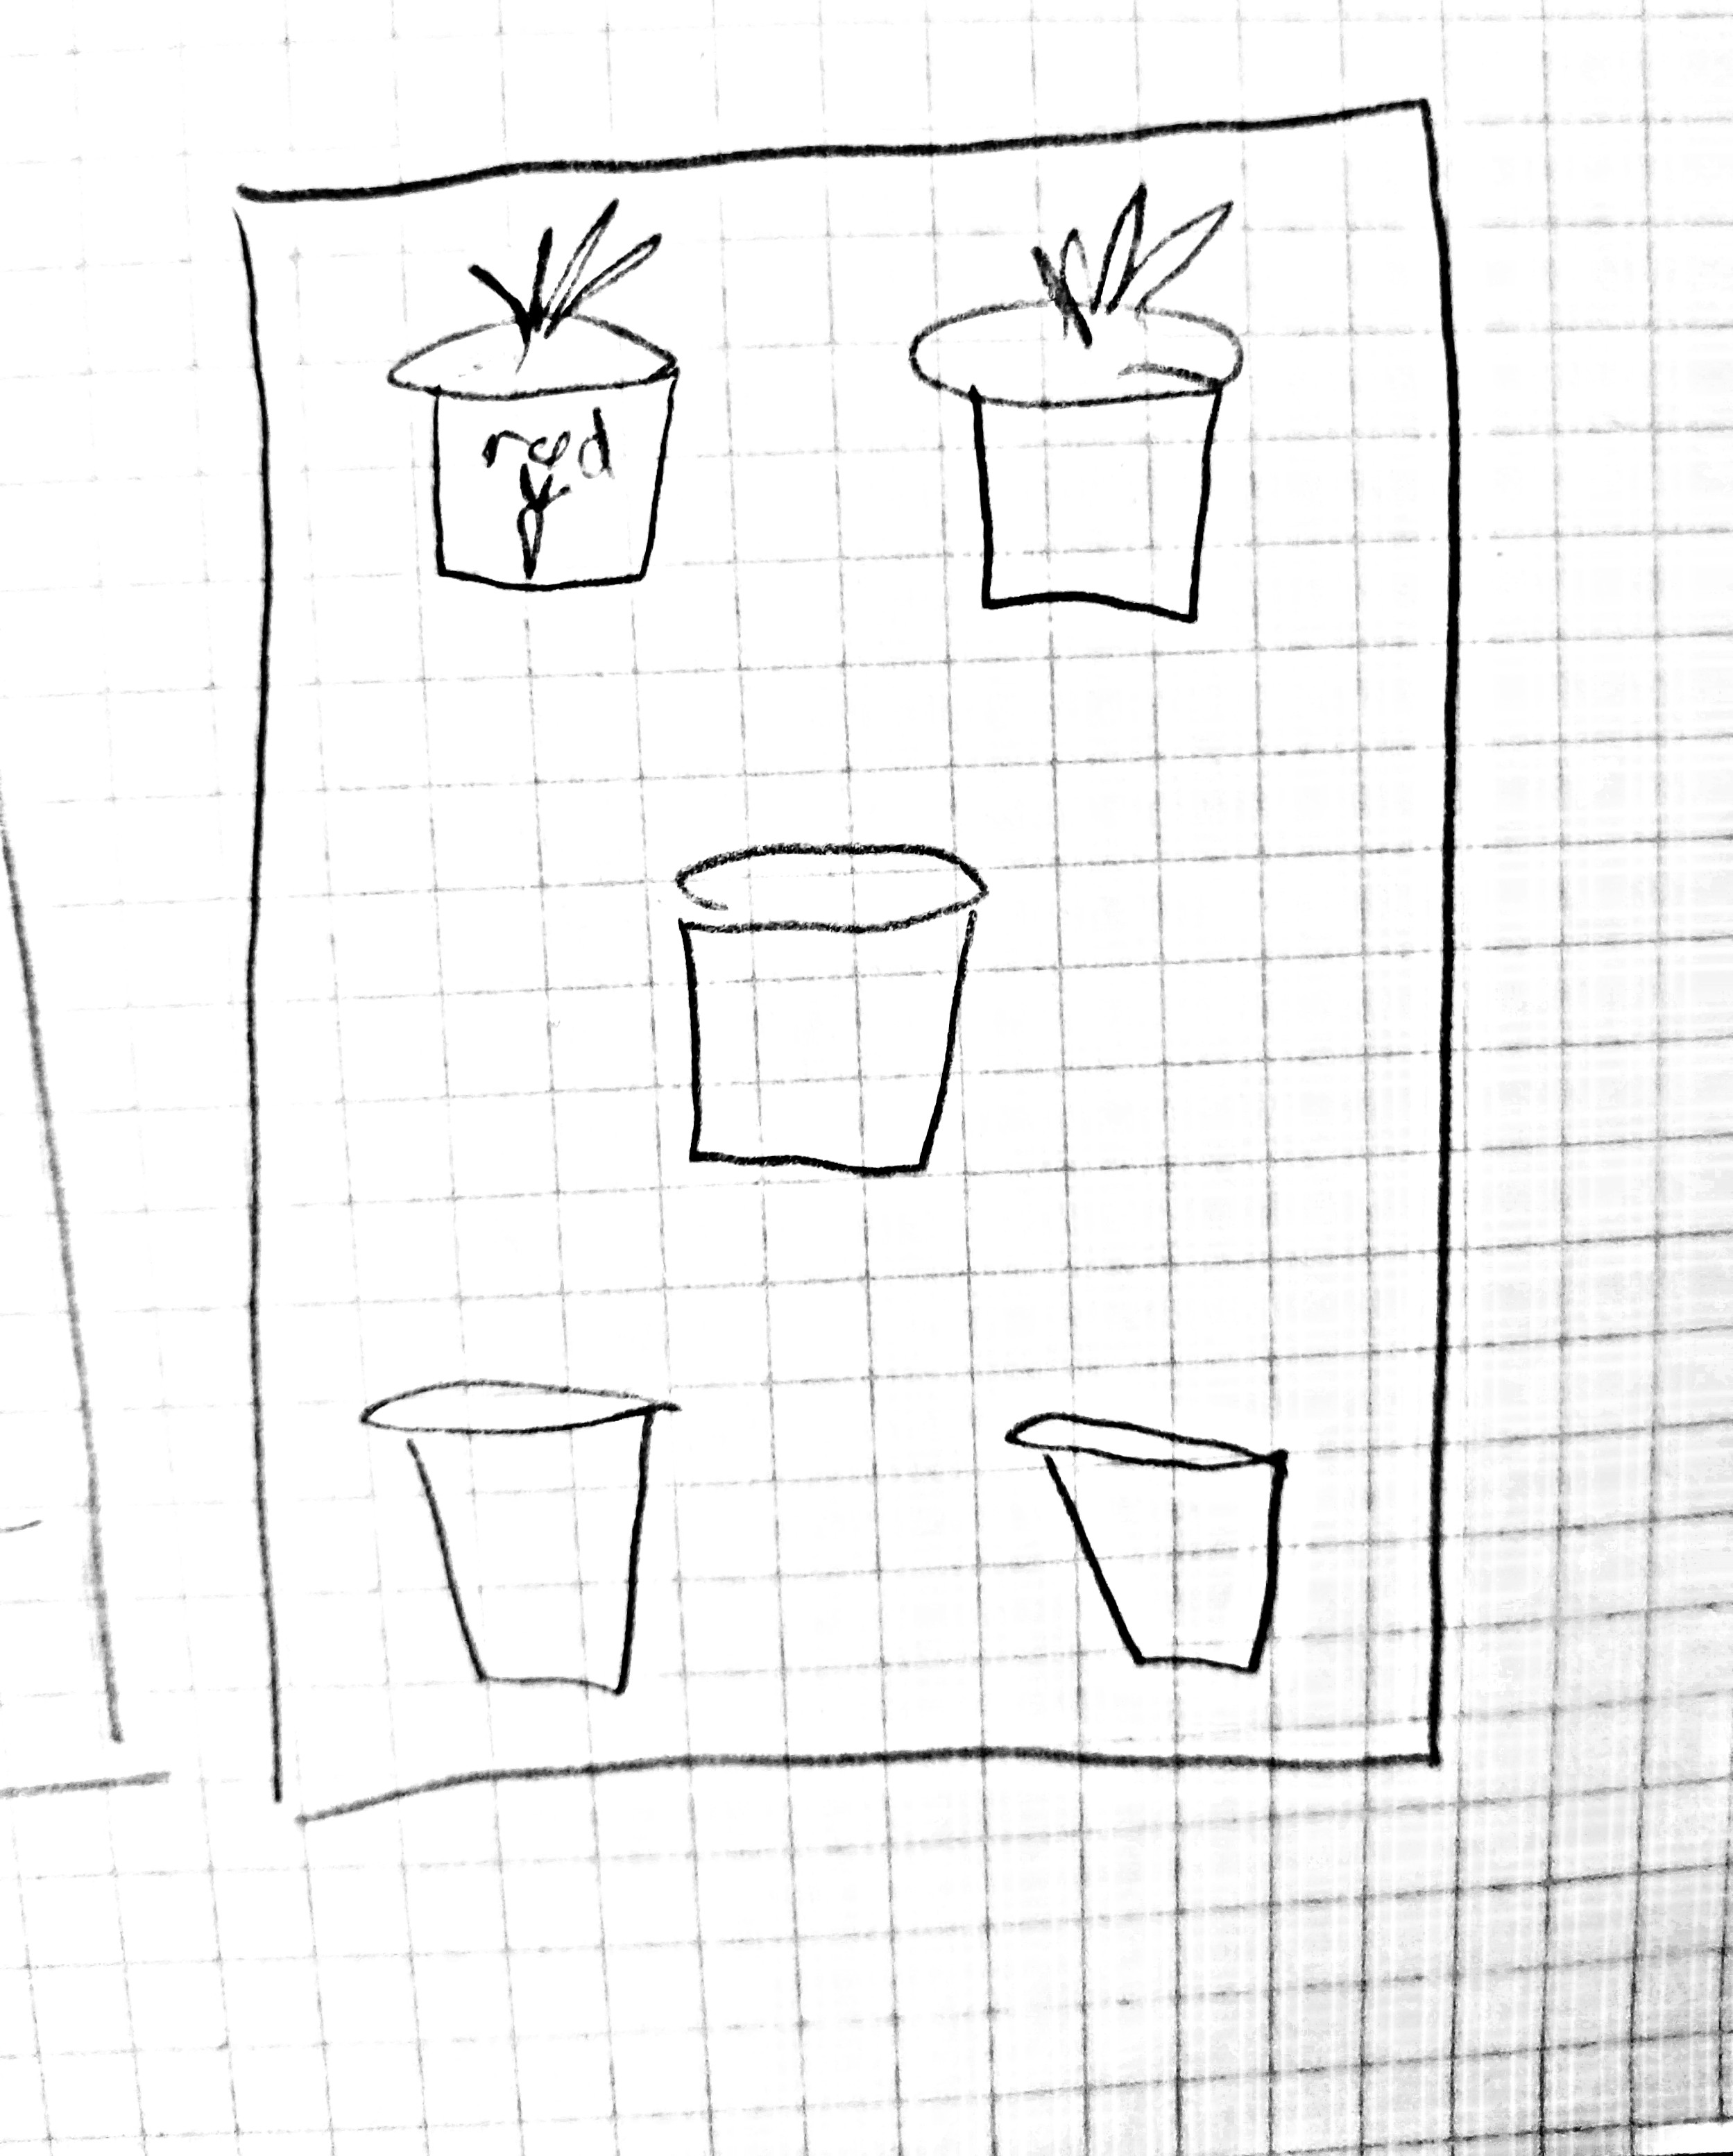
\includegraphics[width=0.6\textwidth]{img/s1-5.jpg}\\
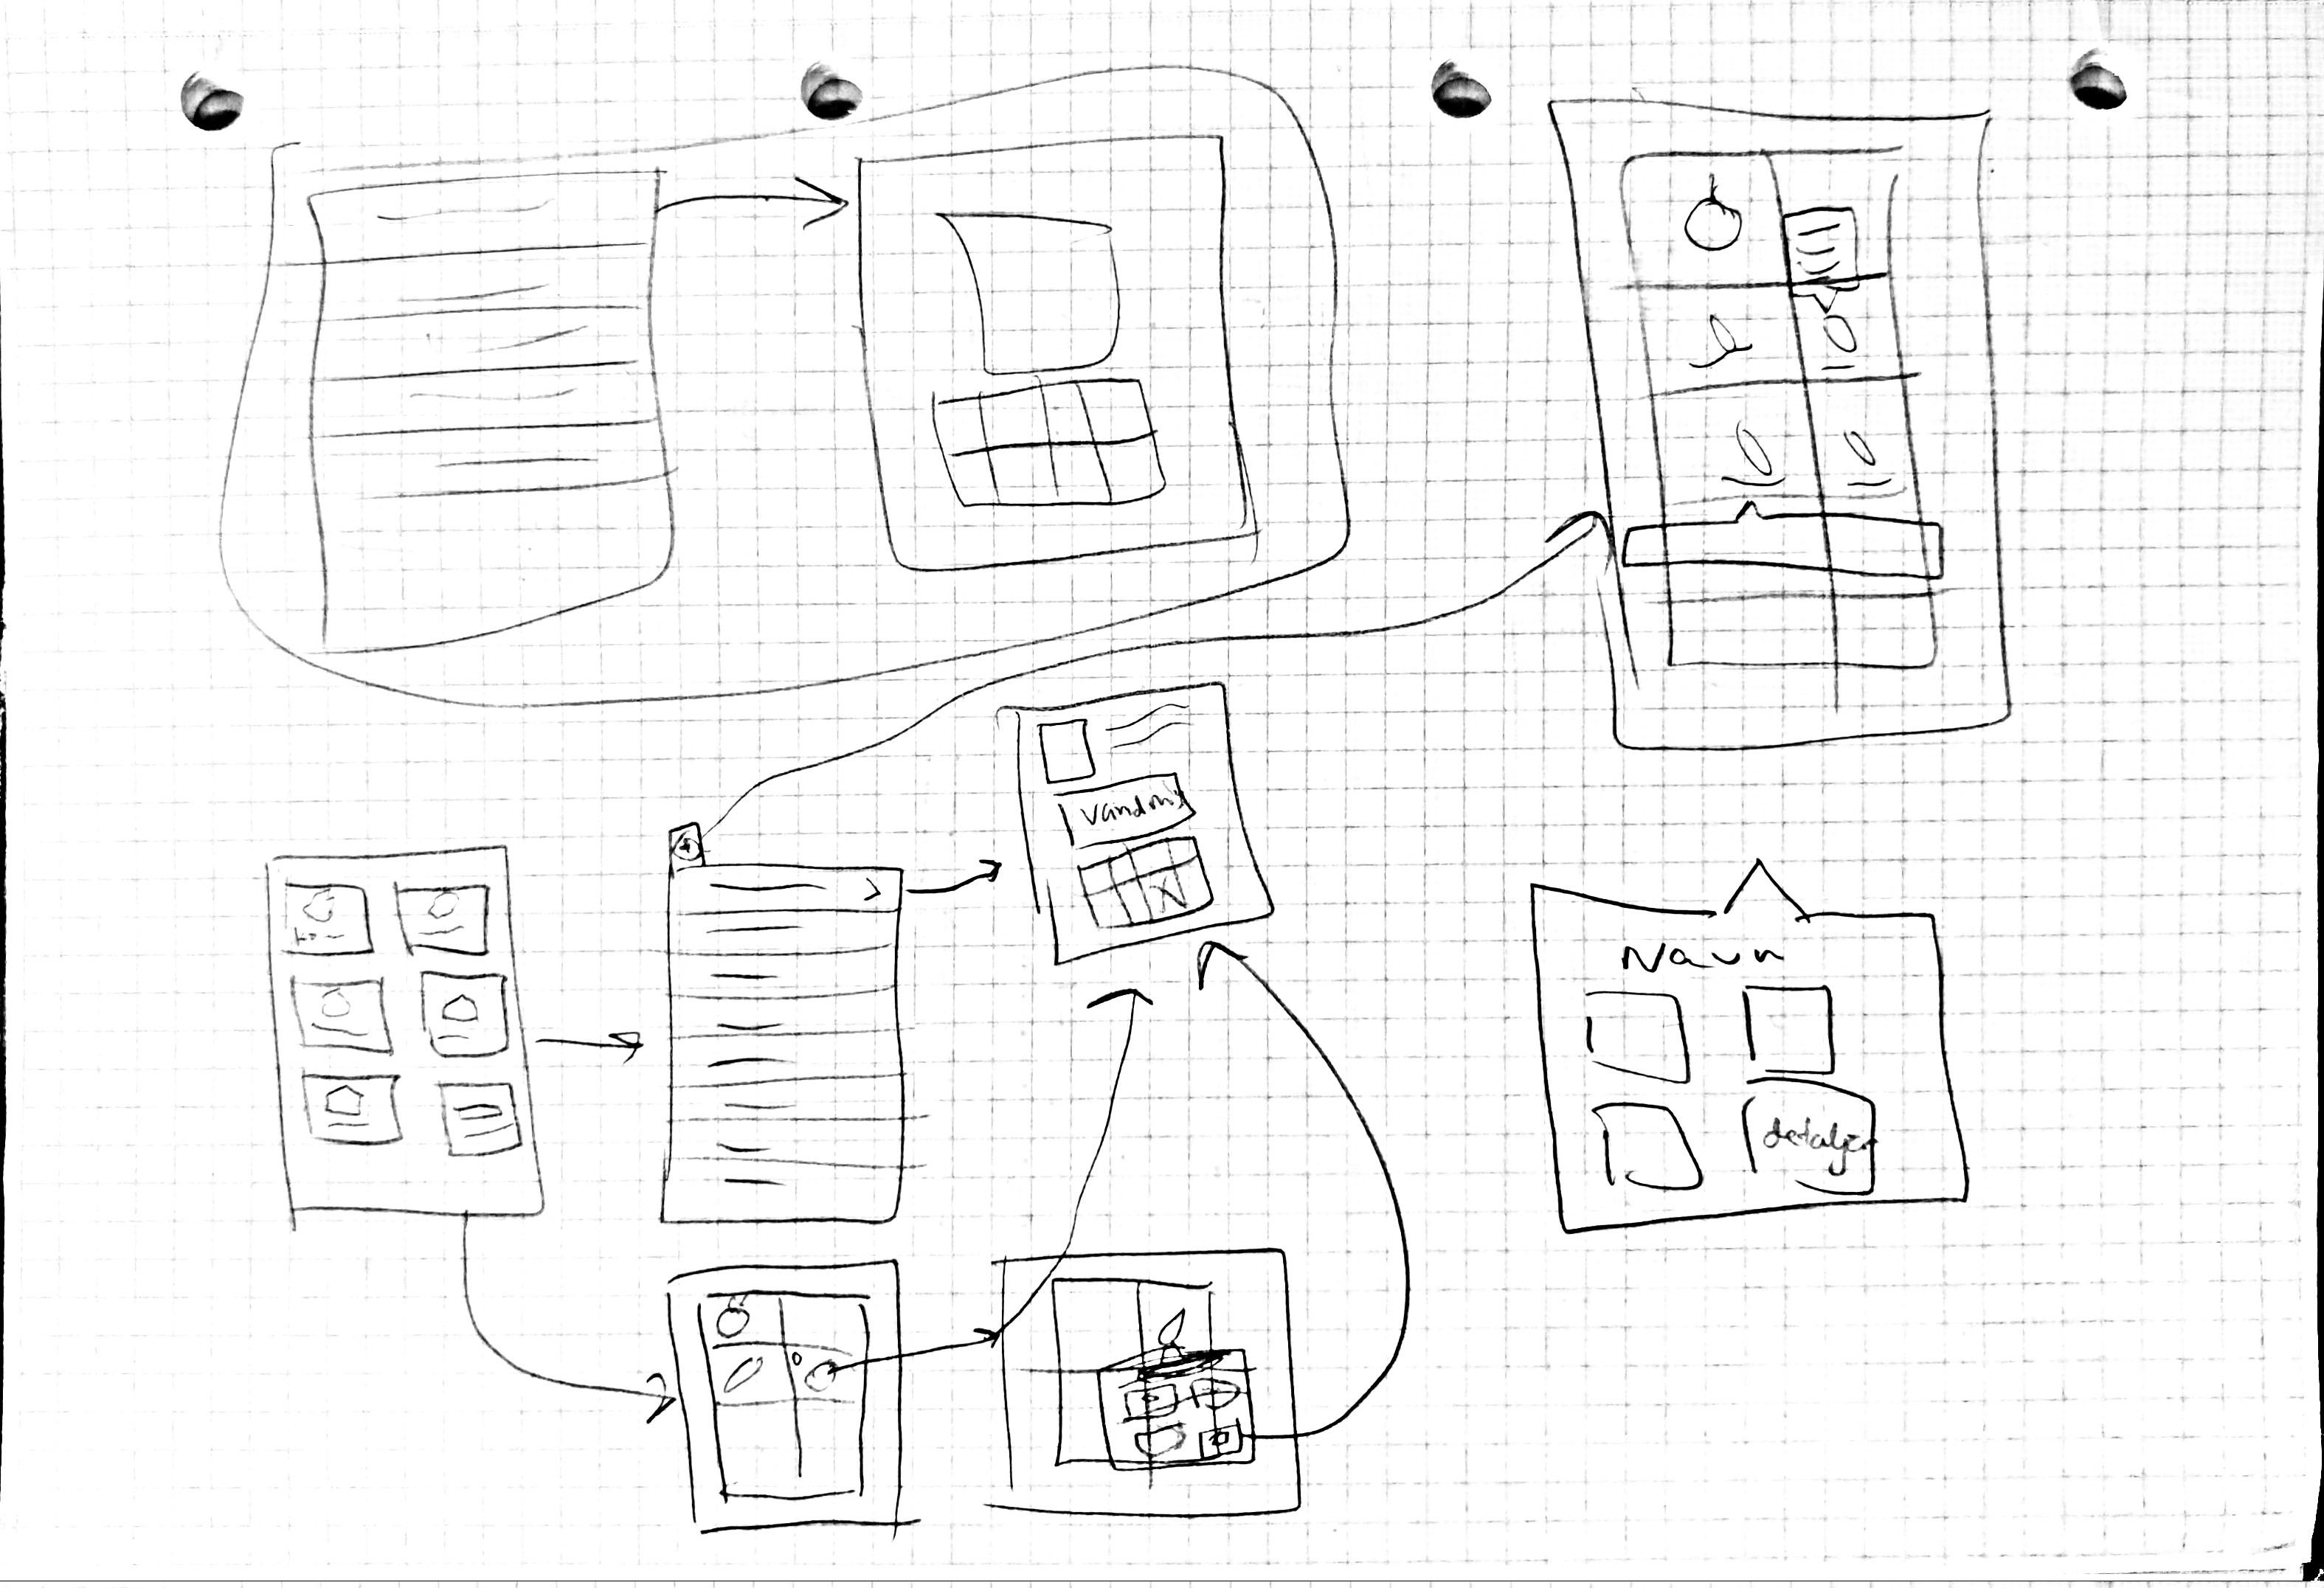
\includegraphics[width=1\textwidth]{img/s1-7.jpg}\\
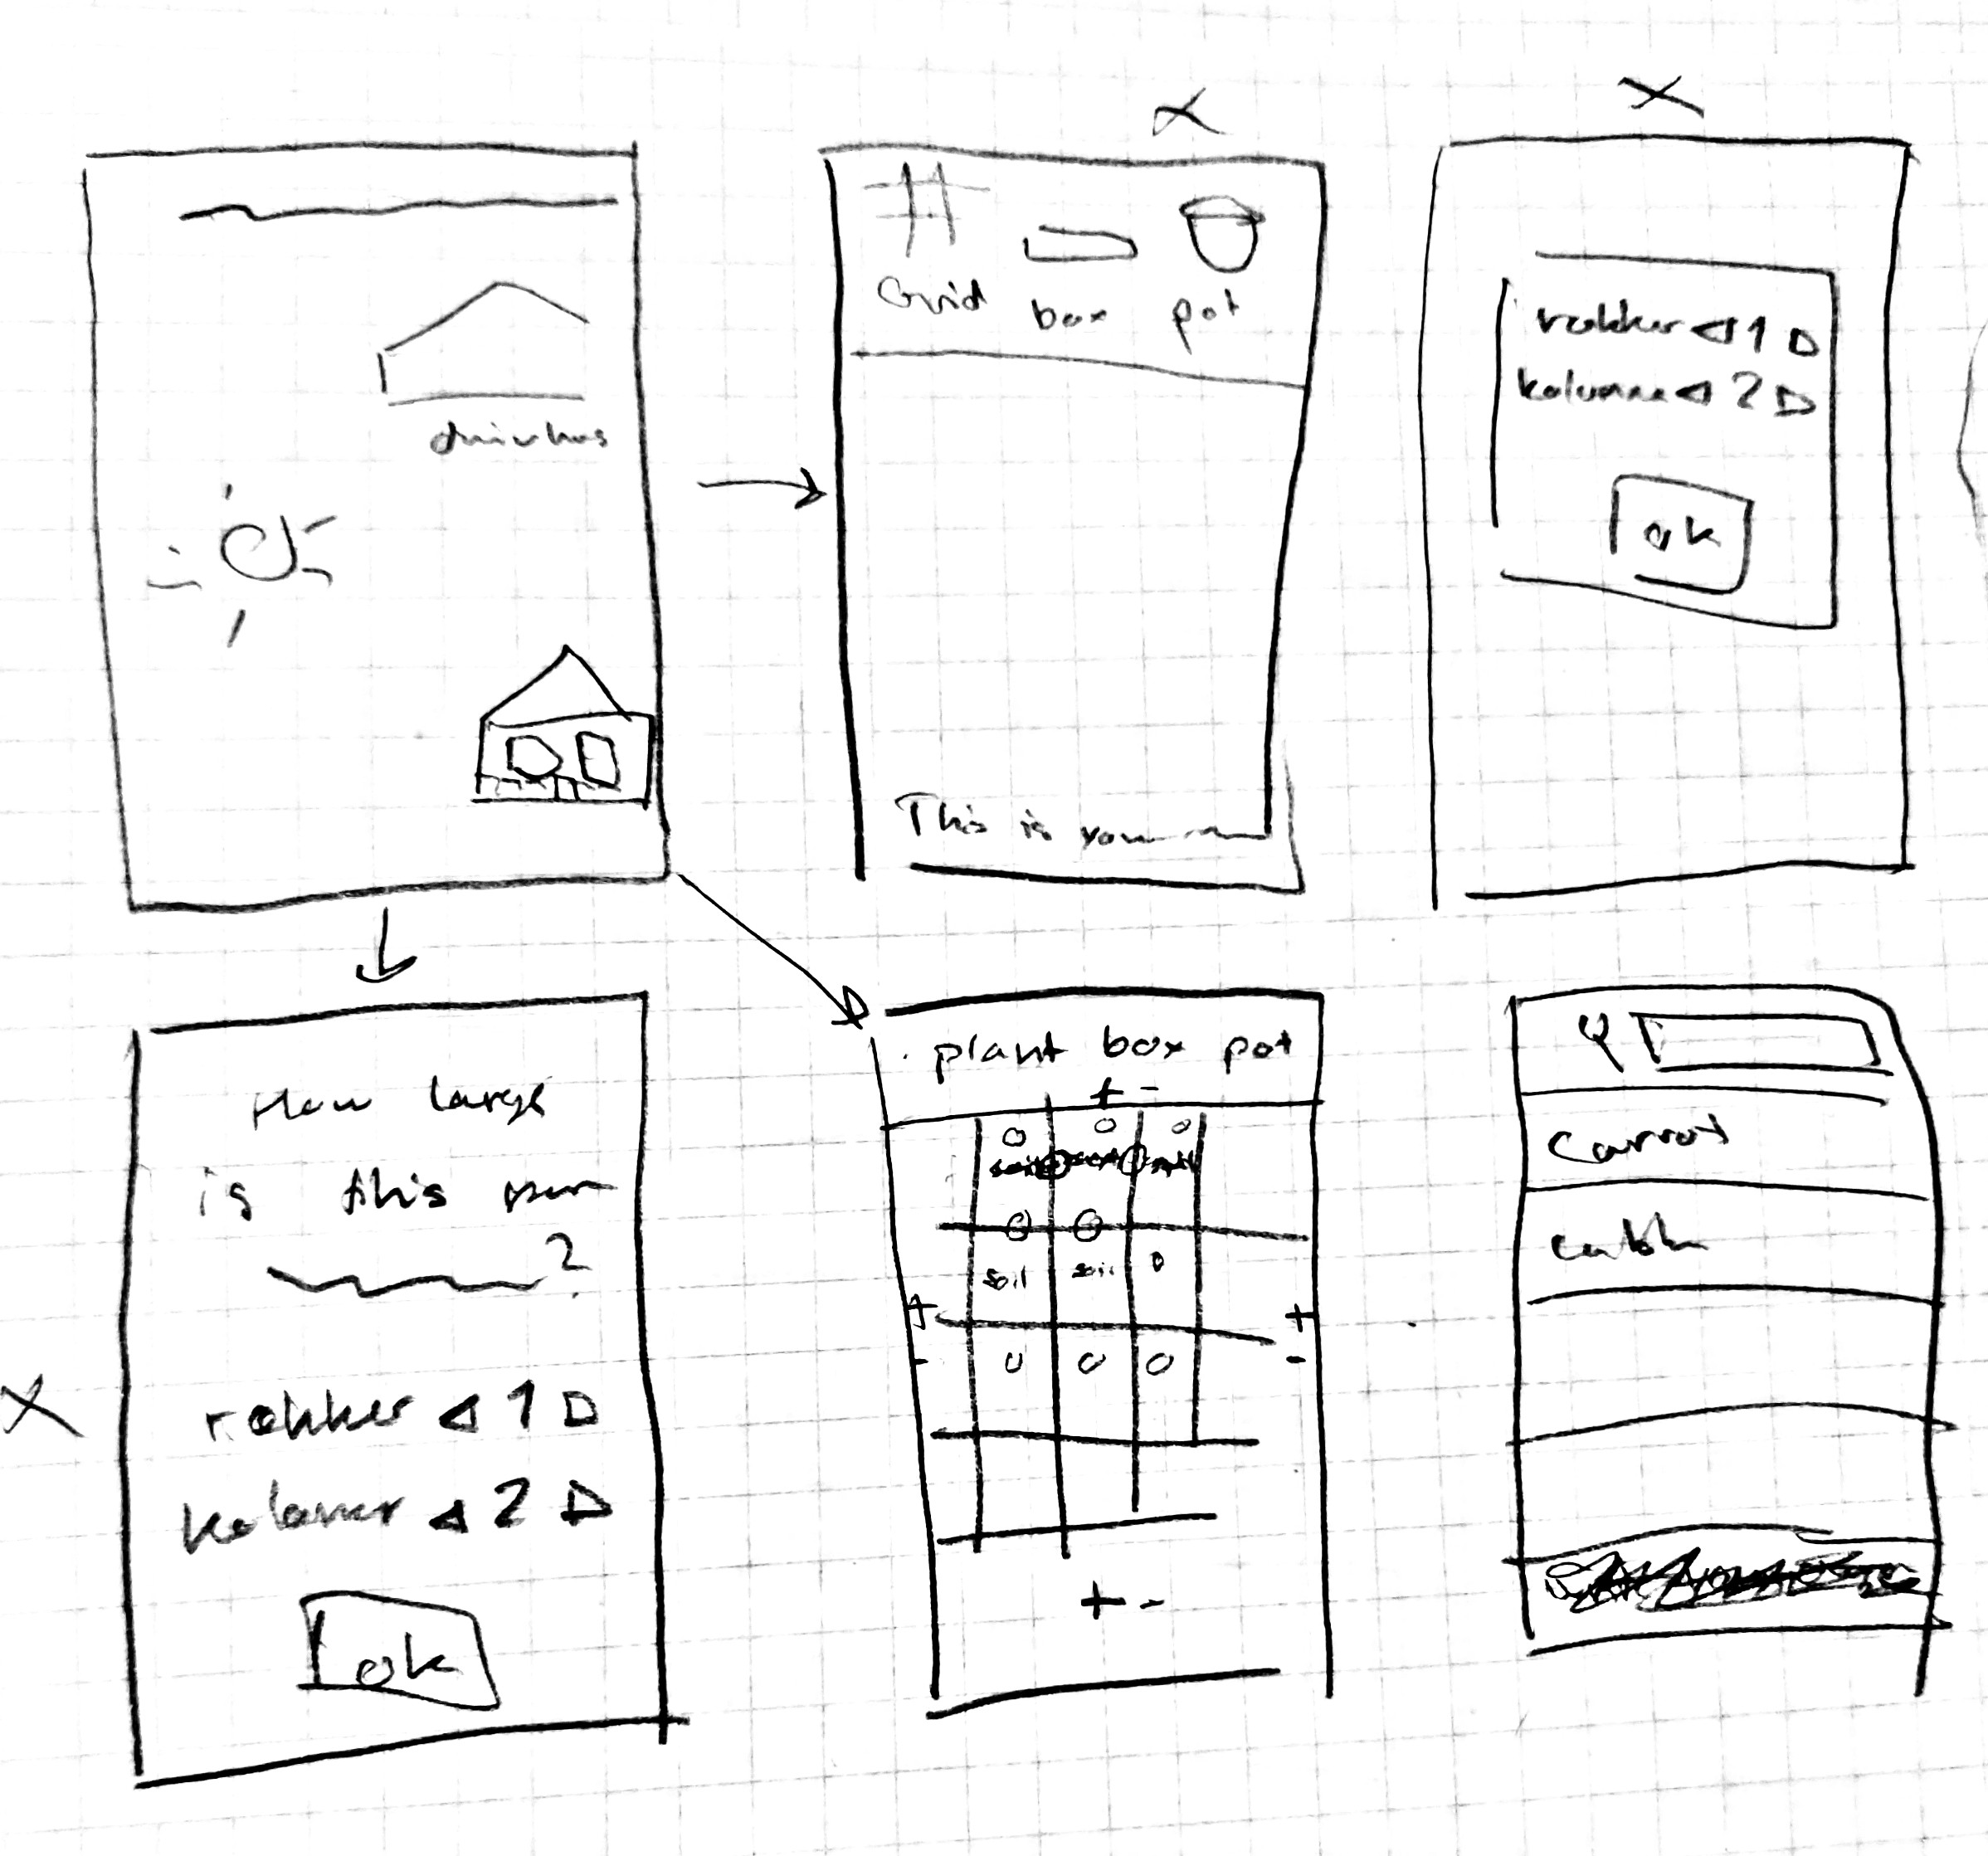
\includegraphics[width=1\textwidth]{img/s1-9.jpg}\\

\subsection{Wireframes}

\begin{itemize}
    \item Navigationen er altid synlig i bunden af skærmen for hurtigt at kunne skife mellem og gå tilbage til forskellige dele af appen
\end{itemize}

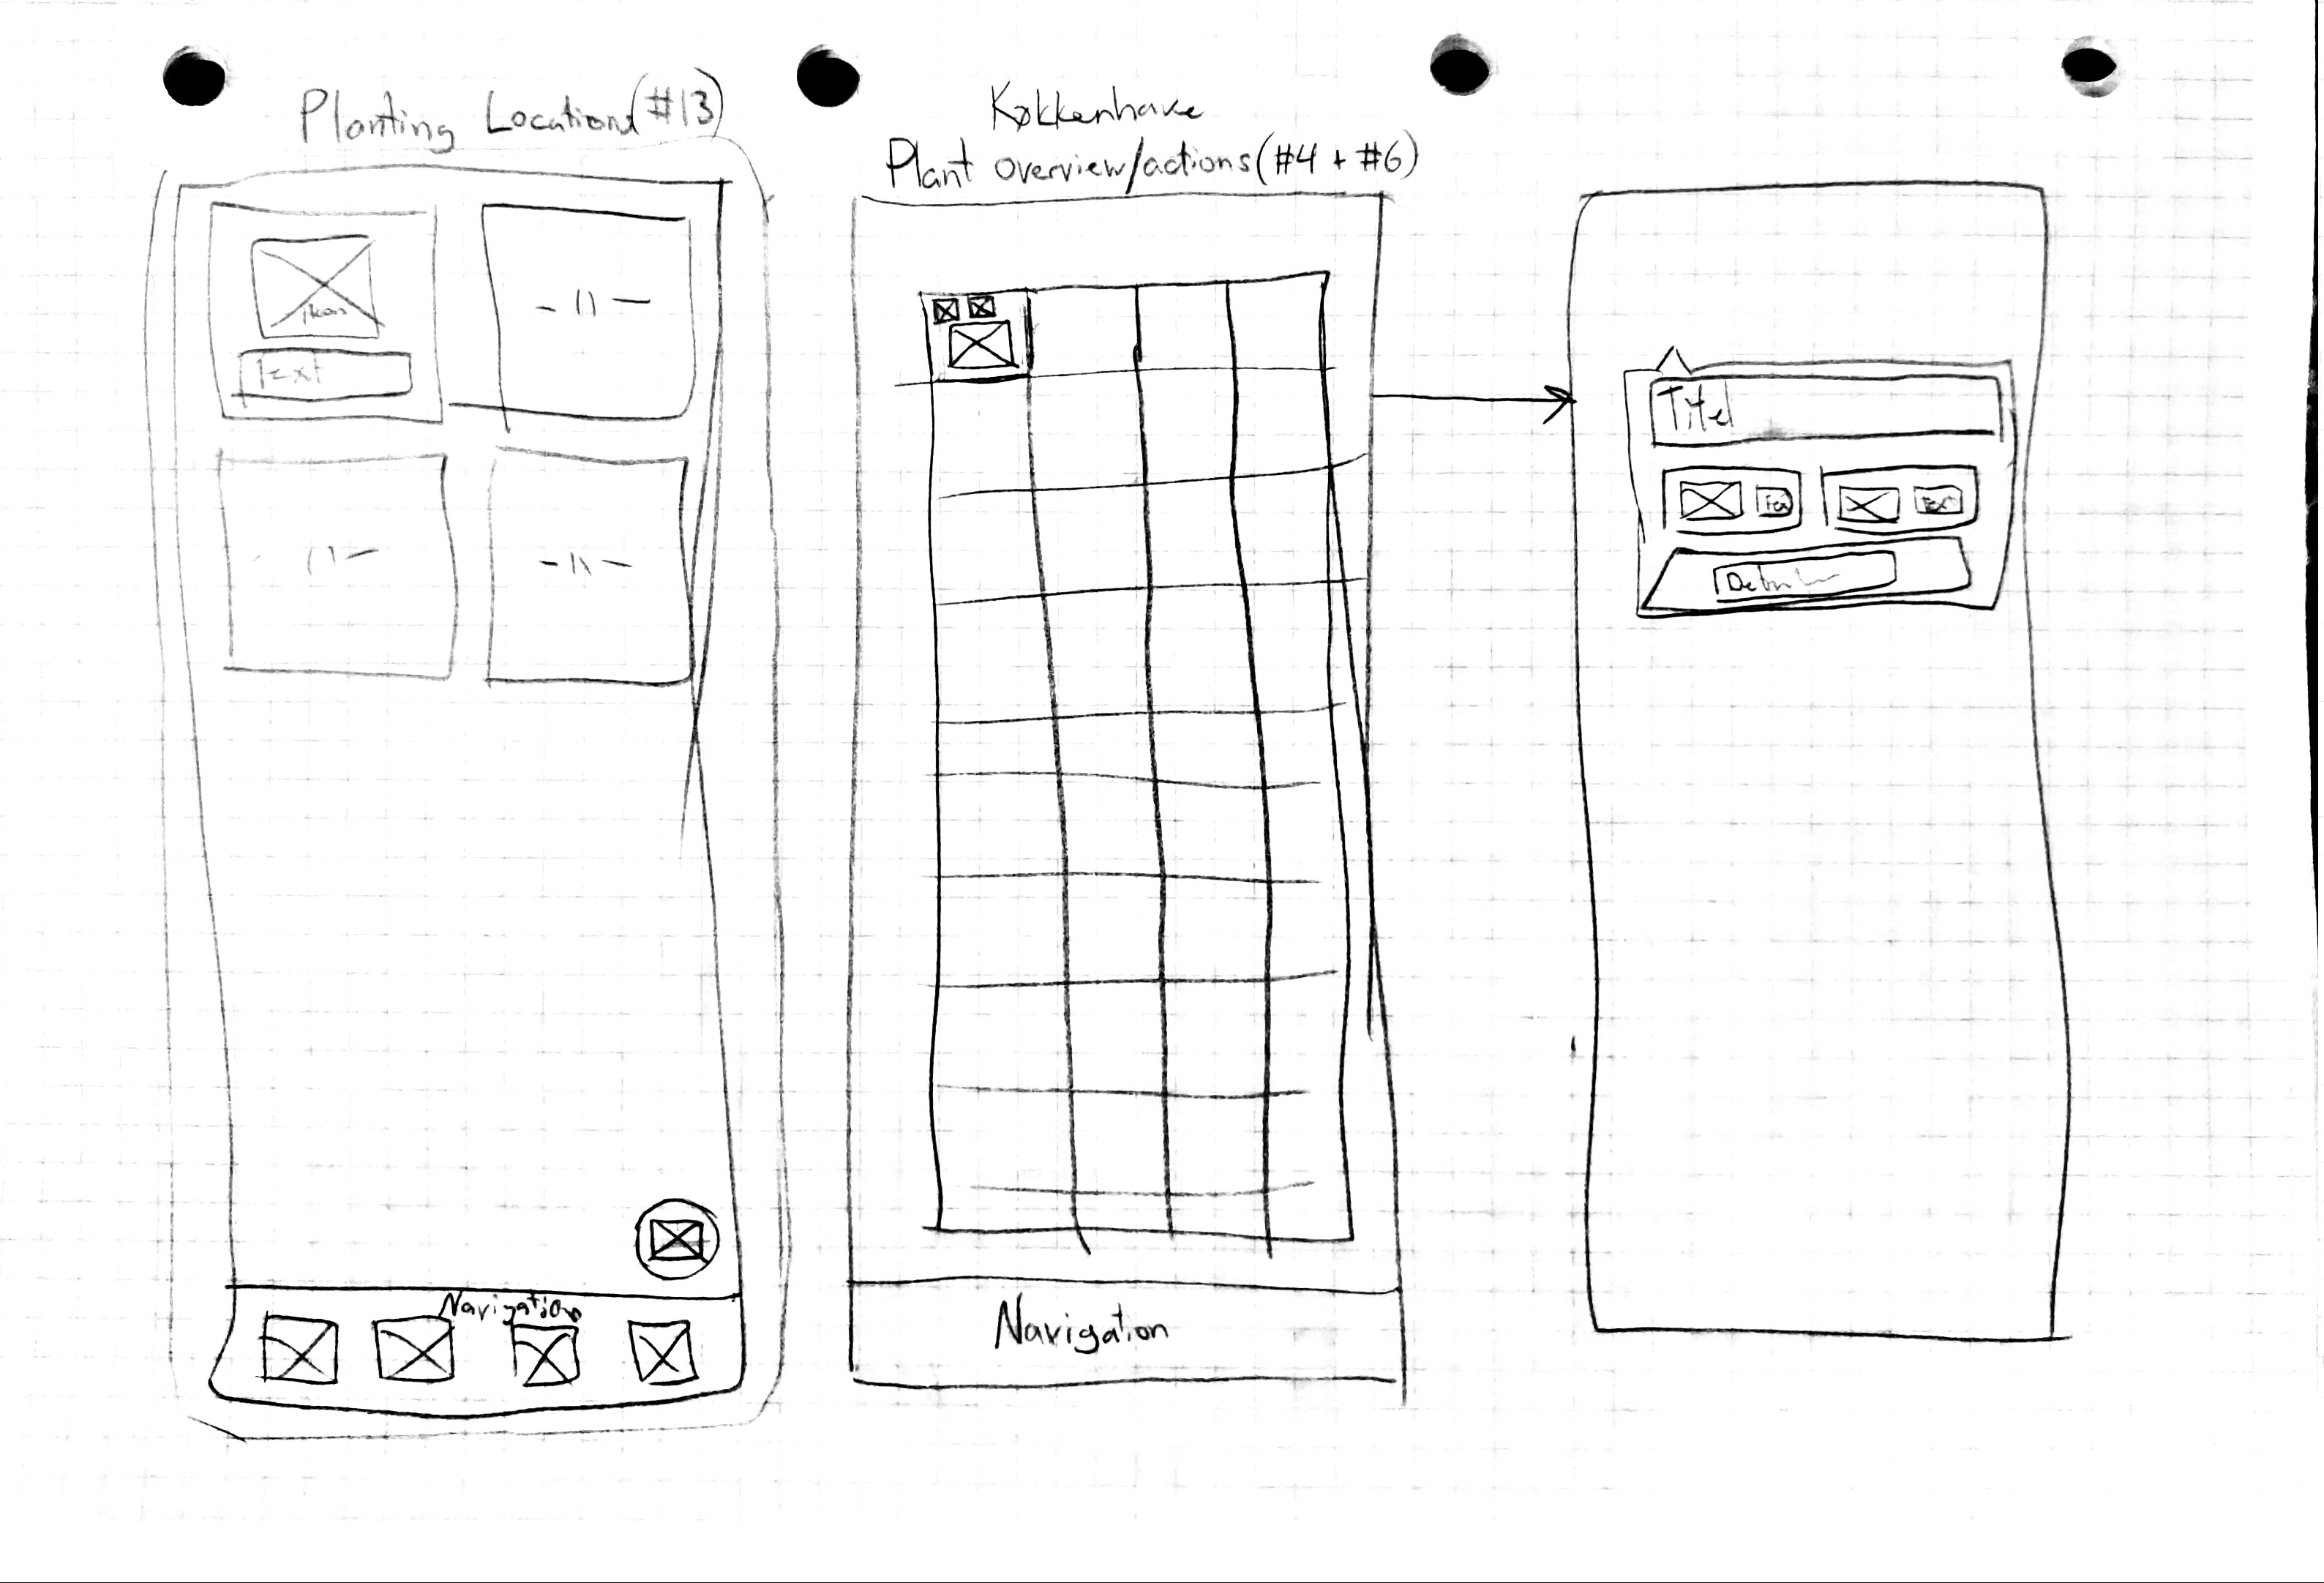
\includegraphics[width=1\textwidth]{img/s1-4.jpg}\\

\begin{itemize}
    \item Grid frem for liste for overblik over hvor planterne er
    \item Store områder bliver indelt i "sider" som man kan bladre imellem, fordi brugeren er vant til at swipe frem for at scrolle til siden
    \item Det bliver inddelt i områder, så brugeren selv kan dele haven op, som de ønsker
    \item Kun ikoner på overblikket af planter for et nemt overblik
\end{itemize}

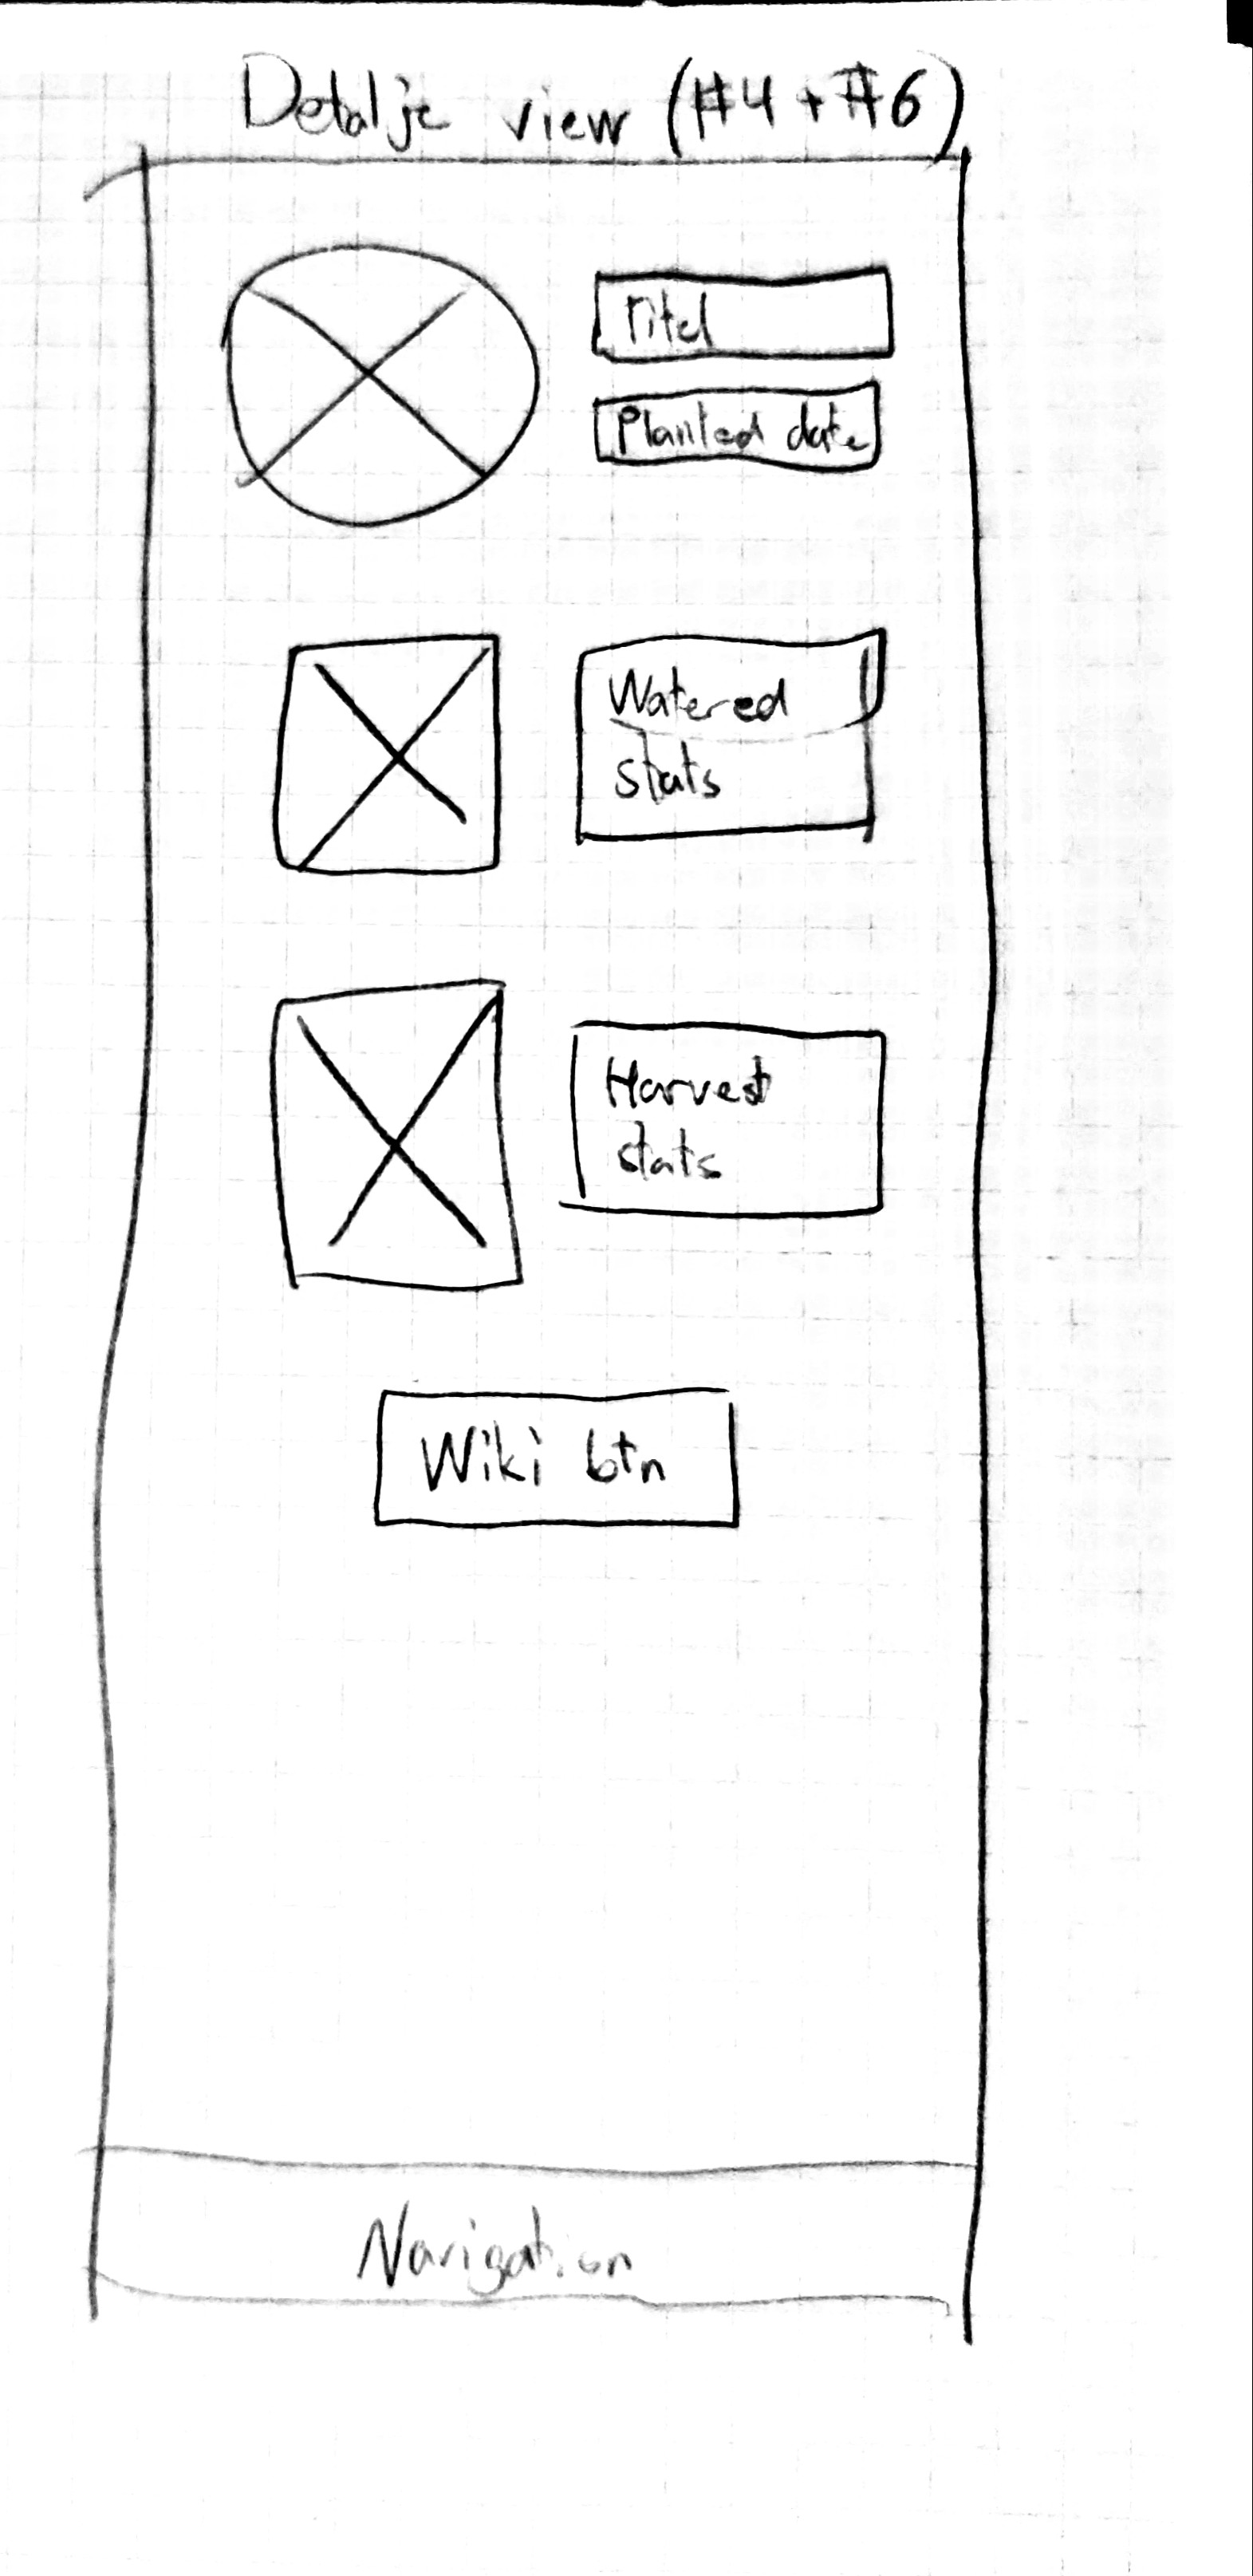
\includegraphics[width=0.5\textwidth]{img/s1-2.jpg}\\

\begin{itemize}
    \item Detajleview hvis man vil vide mere (wiki knap) eller se mere om plantens status
\end{itemize}

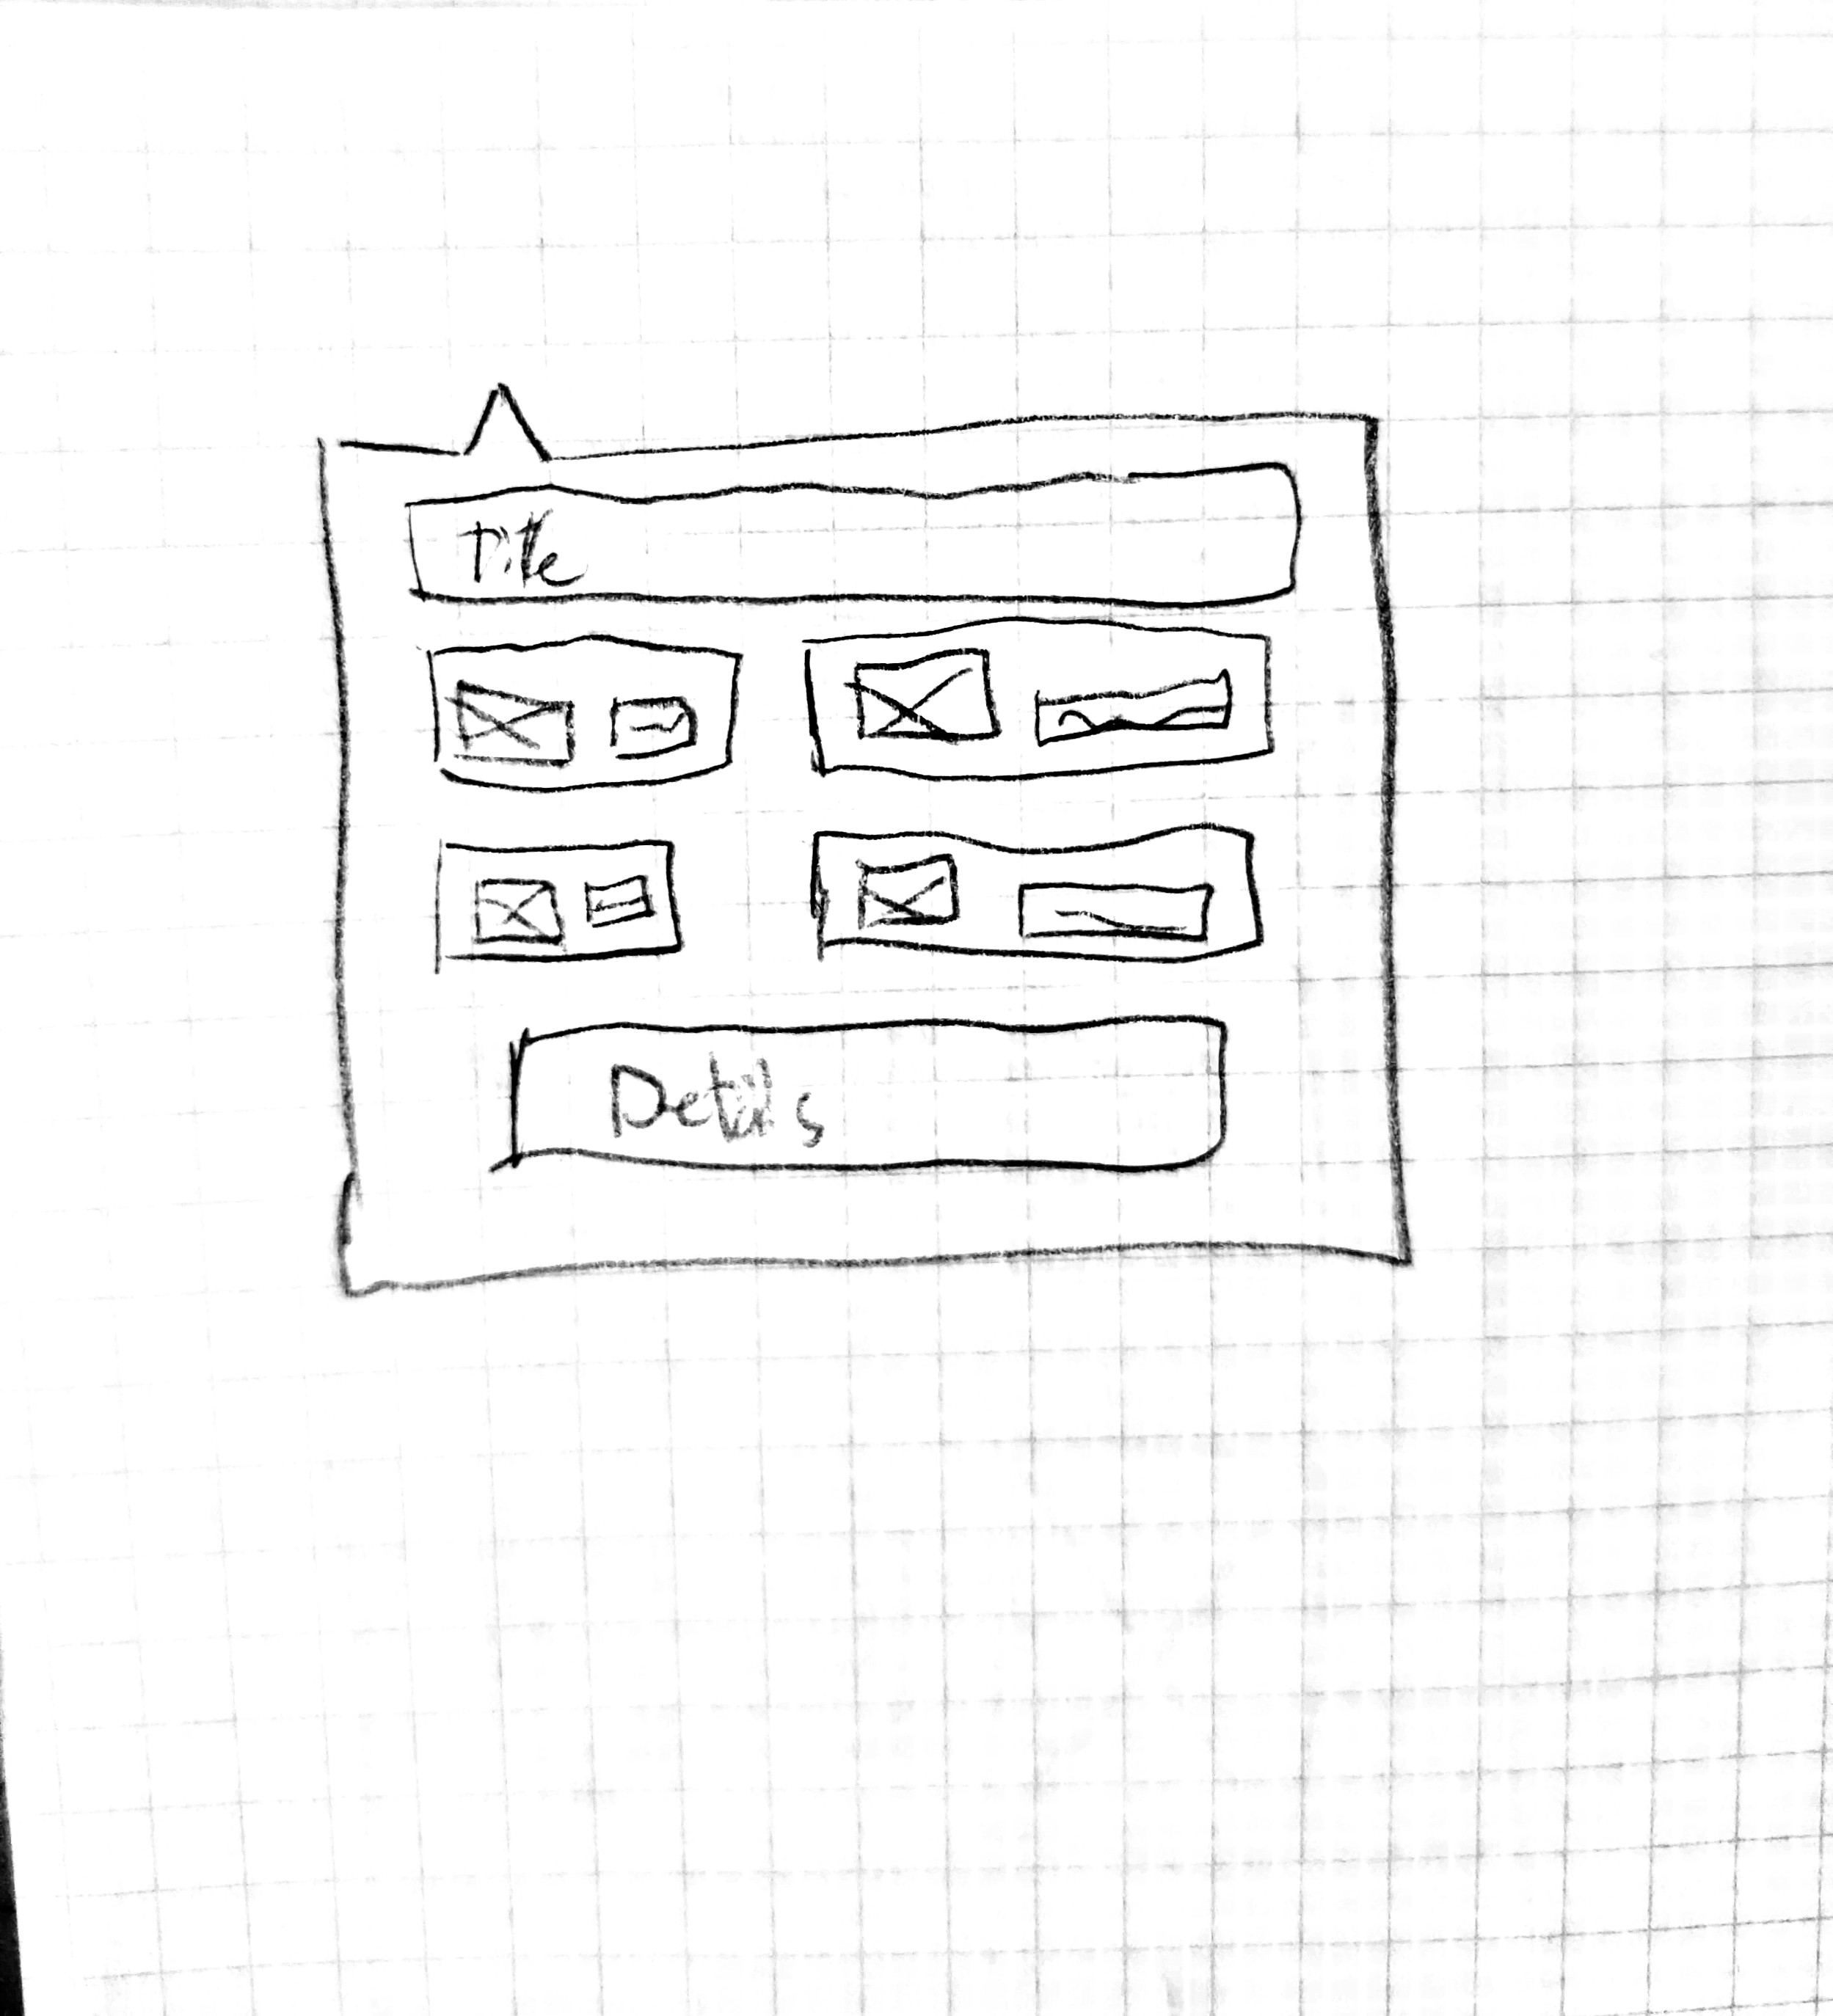
\includegraphics[width=0.5\textwidth]{img/s1-6.jpg}\\

\begin{itemize}
    \item Popup til at udføre "hurtige actions" og for at undgå for mange knapper på griddet så det bliver uoverskueligt og småt
\end{itemize}

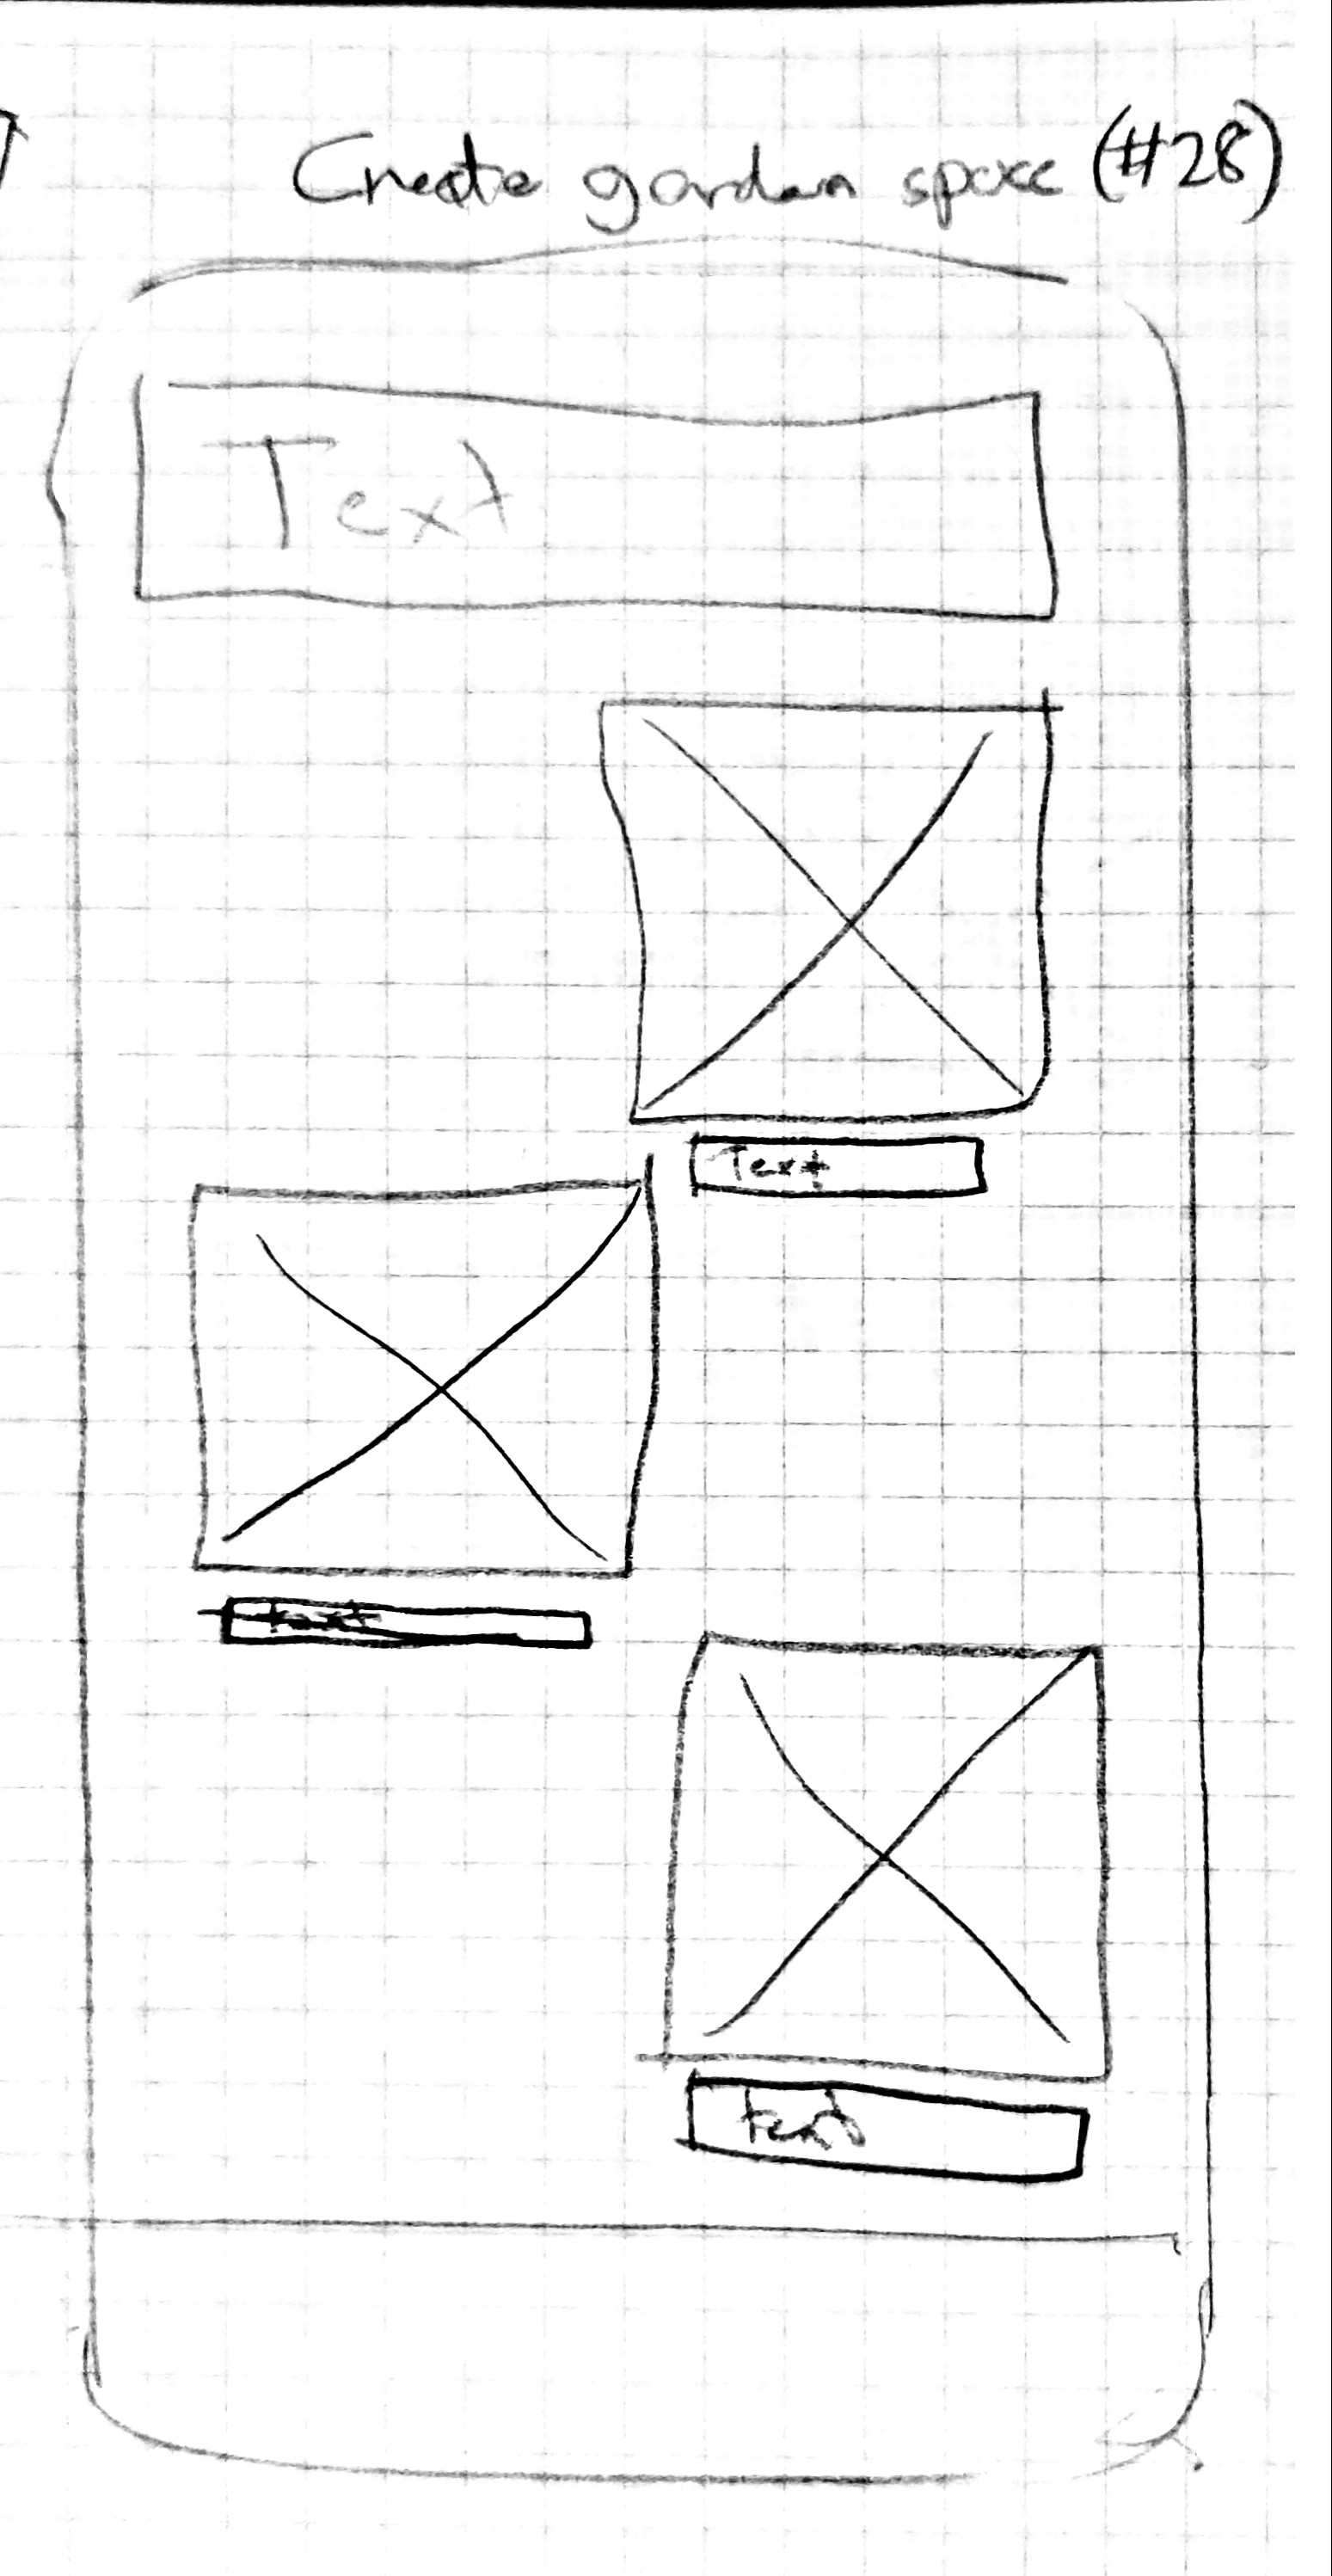
\includegraphics[width=0.5\textwidth]{img/s1-10.jpg}\\

\begin{itemize}
    \item Man starter med at vælge lokation, da det har indflydelse på de actions, man senere skal foretage
    \item Hver location har et ikon samt en tekst
\end{itemize}

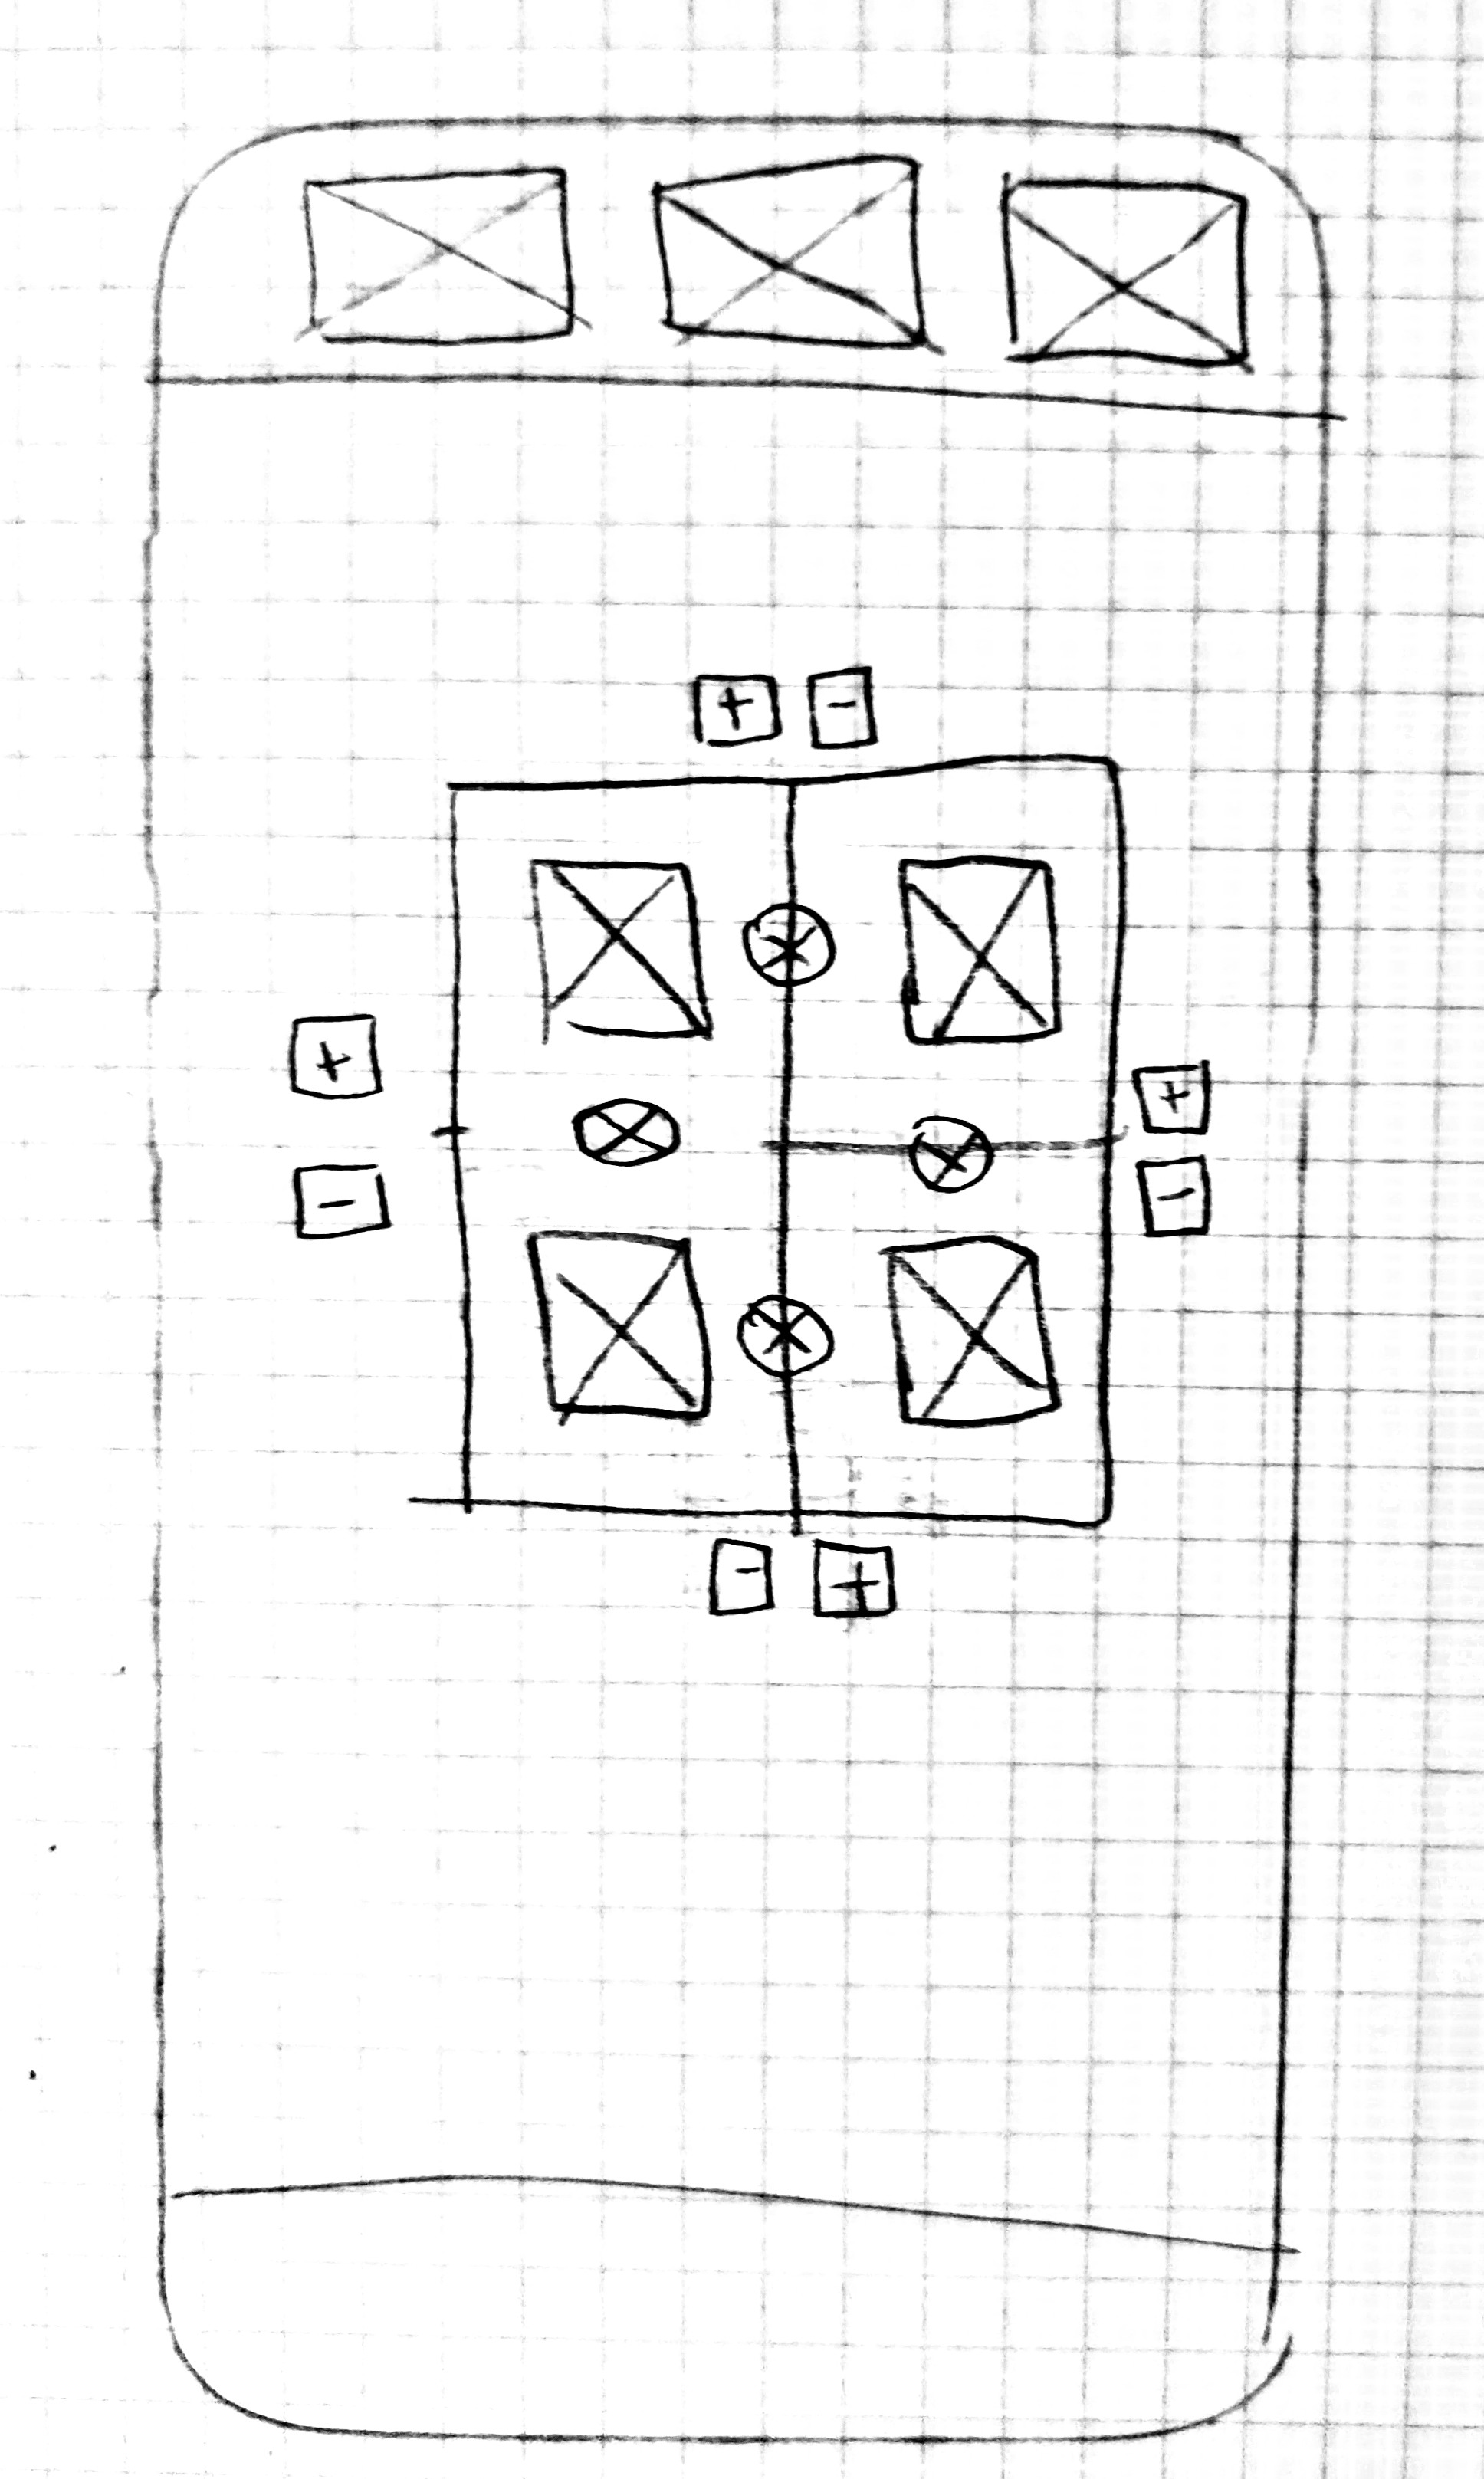
\includegraphics[width=0.5\textwidth]{img/s1-8.jpg}\\

\begin{itemize}
    \item Man kan flette celler, hvis man ikke har lige mange planter i hver kolonne eller række
    \item Man kan tilføje og slette rækker og kolonner for at gøre plads til flere eller færre planter
    \item Man kan hive en plantekasse eller potte ned på griddet for at indikere at der er noget her
\end{itemize}


